% Options for packages loaded elsewhere
\PassOptionsToPackage{unicode}{hyperref}
\PassOptionsToPackage{hyphens}{url}
\PassOptionsToPackage{dvipsnames,svgnames,x11names}{xcolor}
%
\documentclass[
  a4paper,
  DIV=11,
  numbers=noendperiod,
  onepage,
  openany]{scrreprt}

\usepackage{amsmath,amssymb}
\usepackage{iftex}
\ifPDFTeX
  \usepackage[T1]{fontenc}
  \usepackage[utf8]{inputenc}
  \usepackage{textcomp} % provide euro and other symbols
\else % if luatex or xetex
  \usepackage{unicode-math}
  \defaultfontfeatures{Scale=MatchLowercase}
  \defaultfontfeatures[\rmfamily]{Ligatures=TeX,Scale=1}
\fi
\usepackage{lmodern}
\ifPDFTeX\else  
    % xetex/luatex font selection
\fi
% Use upquote if available, for straight quotes in verbatim environments
\IfFileExists{upquote.sty}{\usepackage{upquote}}{}
\IfFileExists{microtype.sty}{% use microtype if available
  \usepackage[]{microtype}
  \UseMicrotypeSet[protrusion]{basicmath} % disable protrusion for tt fonts
}{}
\makeatletter
\@ifundefined{KOMAClassName}{% if non-KOMA class
  \IfFileExists{parskip.sty}{%
    \usepackage{parskip}
  }{% else
    \setlength{\parindent}{0pt}
    \setlength{\parskip}{6pt plus 2pt minus 1pt}}
}{% if KOMA class
  \KOMAoptions{parskip=half}}
\makeatother
\usepackage{xcolor}
\usepackage[lmargin=30mm,rmargin=30mm,tmargin=35mm,bmargin=30mm]{geometry}
\setlength{\emergencystretch}{3em} % prevent overfull lines
\setcounter{secnumdepth}{5}
% Make \paragraph and \subparagraph free-standing
\makeatletter
\ifx\paragraph\undefined\else
  \let\oldparagraph\paragraph
  \renewcommand{\paragraph}{
    \@ifstar
      \xxxParagraphStar
      \xxxParagraphNoStar
  }
  \newcommand{\xxxParagraphStar}[1]{\oldparagraph*{#1}\mbox{}}
  \newcommand{\xxxParagraphNoStar}[1]{\oldparagraph{#1}\mbox{}}
\fi
\ifx\subparagraph\undefined\else
  \let\oldsubparagraph\subparagraph
  \renewcommand{\subparagraph}{
    \@ifstar
      \xxxSubParagraphStar
      \xxxSubParagraphNoStar
  }
  \newcommand{\xxxSubParagraphStar}[1]{\oldsubparagraph*{#1}\mbox{}}
  \newcommand{\xxxSubParagraphNoStar}[1]{\oldsubparagraph{#1}\mbox{}}
\fi
\makeatother

\usepackage{color}
\usepackage{fancyvrb}
\newcommand{\VerbBar}{|}
\newcommand{\VERB}{\Verb[commandchars=\\\{\}]}
\DefineVerbatimEnvironment{Highlighting}{Verbatim}{commandchars=\\\{\}}
% Add ',fontsize=\small' for more characters per line
\usepackage{framed}
\definecolor{shadecolor}{RGB}{241,243,245}
\newenvironment{Shaded}{\begin{snugshade}}{\end{snugshade}}
\newcommand{\AlertTok}[1]{\textcolor[rgb]{0.68,0.00,0.00}{#1}}
\newcommand{\AnnotationTok}[1]{\textcolor[rgb]{0.37,0.37,0.37}{#1}}
\newcommand{\AttributeTok}[1]{\textcolor[rgb]{0.40,0.45,0.13}{#1}}
\newcommand{\BaseNTok}[1]{\textcolor[rgb]{0.68,0.00,0.00}{#1}}
\newcommand{\BuiltInTok}[1]{\textcolor[rgb]{0.00,0.23,0.31}{#1}}
\newcommand{\CharTok}[1]{\textcolor[rgb]{0.13,0.47,0.30}{#1}}
\newcommand{\CommentTok}[1]{\textcolor[rgb]{0.37,0.37,0.37}{#1}}
\newcommand{\CommentVarTok}[1]{\textcolor[rgb]{0.37,0.37,0.37}{\textit{#1}}}
\newcommand{\ConstantTok}[1]{\textcolor[rgb]{0.56,0.35,0.01}{#1}}
\newcommand{\ControlFlowTok}[1]{\textcolor[rgb]{0.00,0.23,0.31}{\textbf{#1}}}
\newcommand{\DataTypeTok}[1]{\textcolor[rgb]{0.68,0.00,0.00}{#1}}
\newcommand{\DecValTok}[1]{\textcolor[rgb]{0.68,0.00,0.00}{#1}}
\newcommand{\DocumentationTok}[1]{\textcolor[rgb]{0.37,0.37,0.37}{\textit{#1}}}
\newcommand{\ErrorTok}[1]{\textcolor[rgb]{0.68,0.00,0.00}{#1}}
\newcommand{\ExtensionTok}[1]{\textcolor[rgb]{0.00,0.23,0.31}{#1}}
\newcommand{\FloatTok}[1]{\textcolor[rgb]{0.68,0.00,0.00}{#1}}
\newcommand{\FunctionTok}[1]{\textcolor[rgb]{0.28,0.35,0.67}{#1}}
\newcommand{\ImportTok}[1]{\textcolor[rgb]{0.00,0.46,0.62}{#1}}
\newcommand{\InformationTok}[1]{\textcolor[rgb]{0.37,0.37,0.37}{#1}}
\newcommand{\KeywordTok}[1]{\textcolor[rgb]{0.00,0.23,0.31}{\textbf{#1}}}
\newcommand{\NormalTok}[1]{\textcolor[rgb]{0.00,0.23,0.31}{#1}}
\newcommand{\OperatorTok}[1]{\textcolor[rgb]{0.37,0.37,0.37}{#1}}
\newcommand{\OtherTok}[1]{\textcolor[rgb]{0.00,0.23,0.31}{#1}}
\newcommand{\PreprocessorTok}[1]{\textcolor[rgb]{0.68,0.00,0.00}{#1}}
\newcommand{\RegionMarkerTok}[1]{\textcolor[rgb]{0.00,0.23,0.31}{#1}}
\newcommand{\SpecialCharTok}[1]{\textcolor[rgb]{0.37,0.37,0.37}{#1}}
\newcommand{\SpecialStringTok}[1]{\textcolor[rgb]{0.13,0.47,0.30}{#1}}
\newcommand{\StringTok}[1]{\textcolor[rgb]{0.13,0.47,0.30}{#1}}
\newcommand{\VariableTok}[1]{\textcolor[rgb]{0.07,0.07,0.07}{#1}}
\newcommand{\VerbatimStringTok}[1]{\textcolor[rgb]{0.13,0.47,0.30}{#1}}
\newcommand{\WarningTok}[1]{\textcolor[rgb]{0.37,0.37,0.37}{\textit{#1}}}

\providecommand{\tightlist}{%
  \setlength{\itemsep}{0pt}\setlength{\parskip}{0pt}}\usepackage{longtable,booktabs,array}
\usepackage{calc} % for calculating minipage widths
% Correct order of tables after \paragraph or \subparagraph
\usepackage{etoolbox}
\makeatletter
\patchcmd\longtable{\par}{\if@noskipsec\mbox{}\fi\par}{}{}
\makeatother
% Allow footnotes in longtable head/foot
\IfFileExists{footnotehyper.sty}{\usepackage{footnotehyper}}{\usepackage{footnote}}
\makesavenoteenv{longtable}
\usepackage{graphicx}
\makeatletter
\def\maxwidth{\ifdim\Gin@nat@width>\linewidth\linewidth\else\Gin@nat@width\fi}
\def\maxheight{\ifdim\Gin@nat@height>\textheight\textheight\else\Gin@nat@height\fi}
\makeatother
% Scale images if necessary, so that they will not overflow the page
% margins by default, and it is still possible to overwrite the defaults
% using explicit options in \includegraphics[width, height, ...]{}
\setkeys{Gin}{width=\maxwidth,height=\maxheight,keepaspectratio}
% Set default figure placement to htbp
\makeatletter
\def\fps@figure{htbp}
\makeatother

\KOMAoption{captions}{tableheading}
\makeatletter
\@ifpackageloaded{tcolorbox}{}{\usepackage[skins,breakable]{tcolorbox}}
\@ifpackageloaded{fontawesome5}{}{\usepackage{fontawesome5}}
\definecolor{quarto-callout-color}{HTML}{909090}
\definecolor{quarto-callout-note-color}{HTML}{0758E5}
\definecolor{quarto-callout-important-color}{HTML}{CC1914}
\definecolor{quarto-callout-warning-color}{HTML}{EB9113}
\definecolor{quarto-callout-tip-color}{HTML}{00A047}
\definecolor{quarto-callout-caution-color}{HTML}{FC5300}
\definecolor{quarto-callout-color-frame}{HTML}{acacac}
\definecolor{quarto-callout-note-color-frame}{HTML}{4582ec}
\definecolor{quarto-callout-important-color-frame}{HTML}{d9534f}
\definecolor{quarto-callout-warning-color-frame}{HTML}{f0ad4e}
\definecolor{quarto-callout-tip-color-frame}{HTML}{02b875}
\definecolor{quarto-callout-caution-color-frame}{HTML}{fd7e14}
\makeatother
\makeatletter
\@ifpackageloaded{bookmark}{}{\usepackage{bookmark}}
\makeatother
\makeatletter
\@ifpackageloaded{caption}{}{\usepackage{caption}}
\AtBeginDocument{%
\ifdefined\contentsname
  \renewcommand*\contentsname{Table of contents}
\else
  \newcommand\contentsname{Table of contents}
\fi
\ifdefined\listfigurename
  \renewcommand*\listfigurename{List of Figures}
\else
  \newcommand\listfigurename{List of Figures}
\fi
\ifdefined\listtablename
  \renewcommand*\listtablename{List of Tables}
\else
  \newcommand\listtablename{List of Tables}
\fi
\ifdefined\figurename
  \renewcommand*\figurename{Figure}
\else
  \newcommand\figurename{Figure}
\fi
\ifdefined\tablename
  \renewcommand*\tablename{Table}
\else
  \newcommand\tablename{Table}
\fi
}
\@ifpackageloaded{float}{}{\usepackage{float}}
\floatstyle{ruled}
\@ifundefined{c@chapter}{\newfloat{codelisting}{h}{lop}}{\newfloat{codelisting}{h}{lop}[chapter]}
\floatname{codelisting}{Listing}
\newcommand*\listoflistings{\listof{codelisting}{List of Listings}}
\makeatother
\makeatletter
\makeatother
\makeatletter
\@ifpackageloaded{caption}{}{\usepackage{caption}}
\@ifpackageloaded{subcaption}{}{\usepackage{subcaption}}
\makeatother

\ifLuaTeX
  \usepackage{selnolig}  % disable illegal ligatures
\fi
\usepackage{bookmark}

\IfFileExists{xurl.sty}{\usepackage{xurl}}{} % add URL line breaks if available
\urlstyle{same} % disable monospaced font for URLs
\hypersetup{
  pdftitle={Curso de FastAPI},
  pdfauthor={Diego Saavedra; Miguel Amaya},
  colorlinks=true,
  linkcolor={blue},
  filecolor={Maroon},
  citecolor={Blue},
  urlcolor={Blue},
  pdfcreator={LaTeX via pandoc}}


\title{Curso de FastAPI}
\author{Diego Saavedra \and Miguel Amaya}
\date{Jul 26, 2024}

\begin{document}
\maketitle

\renewcommand*\contentsname{Table of contents}
{
\hypersetup{linkcolor=}
\setcounter{tocdepth}{2}
\tableofcontents
}

\bookmarksetup{startatroot}

\chapter{Bienvenido}\label{bienvenido}

¡Bienvenido al Curso Completo de FastAPI!

En este curso, exploraremos todo, desde los fundamentos hasta las
aplicaciones prácticas.

\section{¿De qué trata este curso?}\label{de-quuxe9-trata-este-curso}

Este curso completo me llevará desde los fundamentos básicos de la
programación hasta la construcción de aplicaciones prácticas utilizando
los frameworks Django y la biblioteca de React.

A través de una combinación de teoría y ejercicios prácticos, me
sumergiré en los conceptos esenciales del desarrollo web y avanzaré
hacia la creación de proyectos del mundo real.

Desde la configuración del entorno de desarrollo hasta la construcción
de una aplicación web de pila completa, este curso me proporcionará una
comprensión sólida y experiencia práctica con FastAPI.

\section{¿Para quién es este curso?}\label{para-quiuxe9n-es-este-curso}

Este curso está diseñado para principiantes y aquellos con poca o
ninguna experiencia en programación.

Ya sea que sea un estudiante curioso, un profesional que busca cambiar
de carrera o simplemente alguien que quiere aprender desarrollo web,
este curso es para usted. Desde adolescentes hasta adultos, todos son
bienvenidos a participar y explorar el emocionante mundo del desarrollo
web con FastAPI.

\section{¿Cómo contribuir?}\label{cuxf3mo-contribuir}

Valoramos su contribución a este curso. Si encuentra algún error, desea
sugerir mejoras o agregar contenido adicional, me encantaría saber de
usted.

Puede contribuir a través del repositorio en linea, donde puede
compartir sus comentarios y sugerencias.

Juntos, podemos mejorar continuamente este recurso educativo para
beneficiar a la comunidad de estudiantes y entusiastas de la
programación.

Este ebook ha sido creado con el objetivo de proporcionar acceso
gratuito y universal al conocimiento.

Estará disponible en línea para cualquier persona, sin importar su
ubicación o circunstancias, para acceder y aprender a su propio ritmo.

Puede descargarlo en formato PDF, Epub o verlo en línea en cualquier
momento y lugar.

Esperamos que disfrute este emocionante viaje de aprendizaje y
descubrimiento en el mundo del desarrollo web con FastAPI!

\part{Unidad 1: Introducción a Python}

\chapter{Configuración y Sintaxis
básica}\label{configuraciuxf3n-y-sintaxis-buxe1sica}

\begin{figure}[H]

{\centering \includegraphics[width=2.08333in,height=\textheight]{index_files/mediabag/1200px-Python-logo-n.png}

}

\caption{Python}

\end{figure}%

Para empezar a trabajar con python es necesario tener instalado el
interprete de python en tu computadora. Para ello puedes descargarlo
desde la página oficial de python \url{https://www.python.org/}.

Una vez instalado, puedes abrir una terminal y escribir \textbf{python}
para abrir el interprete de python. Si ves un mensaje similar a este:

\begin{Shaded}
\begin{Highlighting}[]
\NormalTok{Python }\FloatTok{3.12.4}\NormalTok{ (main, Jun  }\DecValTok{7} \DecValTok{2024}\NormalTok{, }\DecValTok{00}\NormalTok{:}\DecValTok{00}\NormalTok{:}\DecValTok{00}\NormalTok{) [GCC }\FloatTok{14.1.1} \DecValTok{20240607}\NormalTok{ (Red Hat }\FloatTok{14.1.1}\OperatorTok{{-}}\DecValTok{5}\NormalTok{)] on linux}
\NormalTok{Type }\StringTok{"help"}\NormalTok{, }\StringTok{"copyright"}\NormalTok{, }\StringTok{"credits"} \KeywordTok{or} \StringTok{"license"} \ControlFlowTok{for}\NormalTok{ more information.}
\OperatorTok{\textgreater{}\textgreater{}\textgreater{}}
\end{Highlighting}
\end{Shaded}

Significa que python está instalado correctamente en tu computadora.

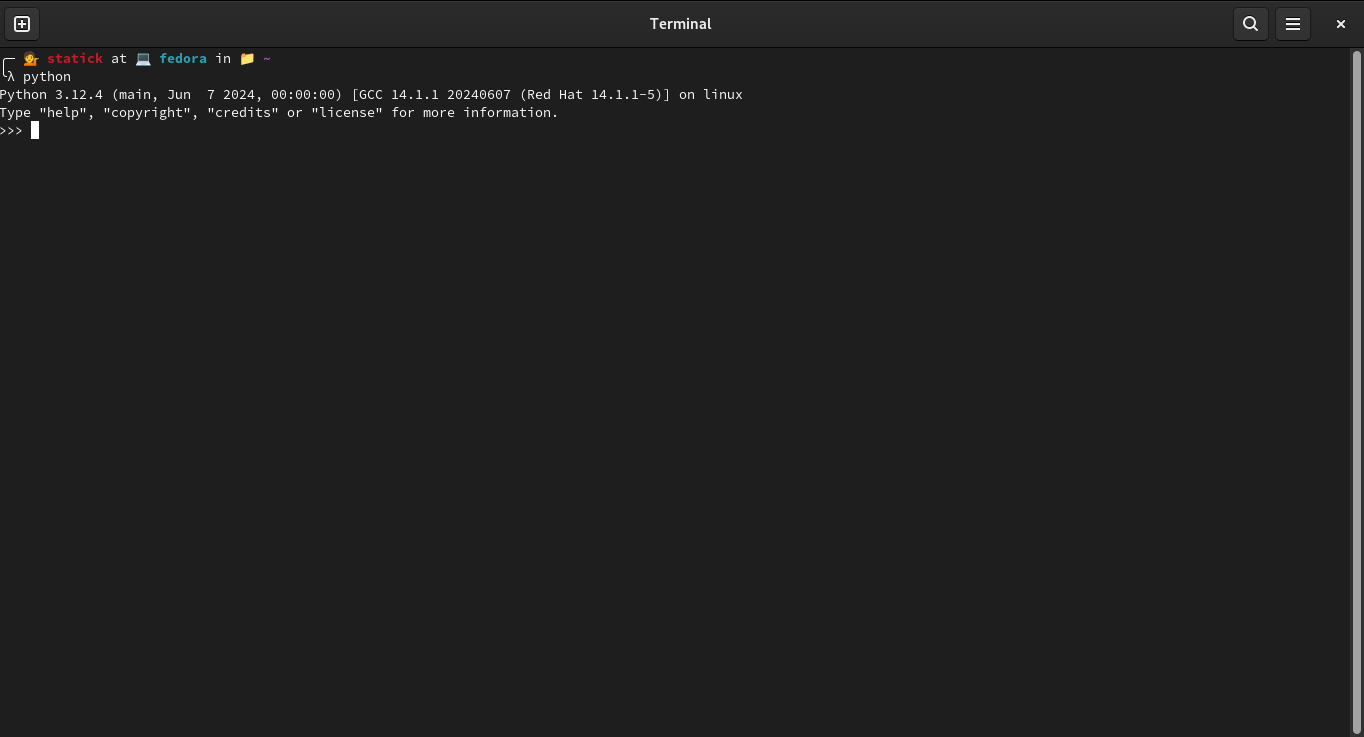
\includegraphics{unidades/unidad1/images/paste-1.png}

Para salir del interprete de python puedes escribir \textbf{exit()} o
\textbf{Ctrl + D}.

\section{Sintaxis básica}\label{sintaxis-buxe1sica}

Python es un lenguaje de programación interpretado, lo que significa que
el código se ejecuta línea por línea. A continuación se muestra un
ejemplo de un programa simple en python:

\begin{Shaded}
\begin{Highlighting}[]
\CommentTok{\# Este es un comentario}
\BuiltInTok{print}\NormalTok{(}\StringTok{"Hola Mundo!"}\NormalTok{)}
\end{Highlighting}
\end{Shaded}

Para ejecutar este programa, puedes guardar el código en un archivo con
extensión \textbf{.py} y ejecutarlo desde la terminal con el comando
\textbf{python nombre\_del\_archivo.py}.

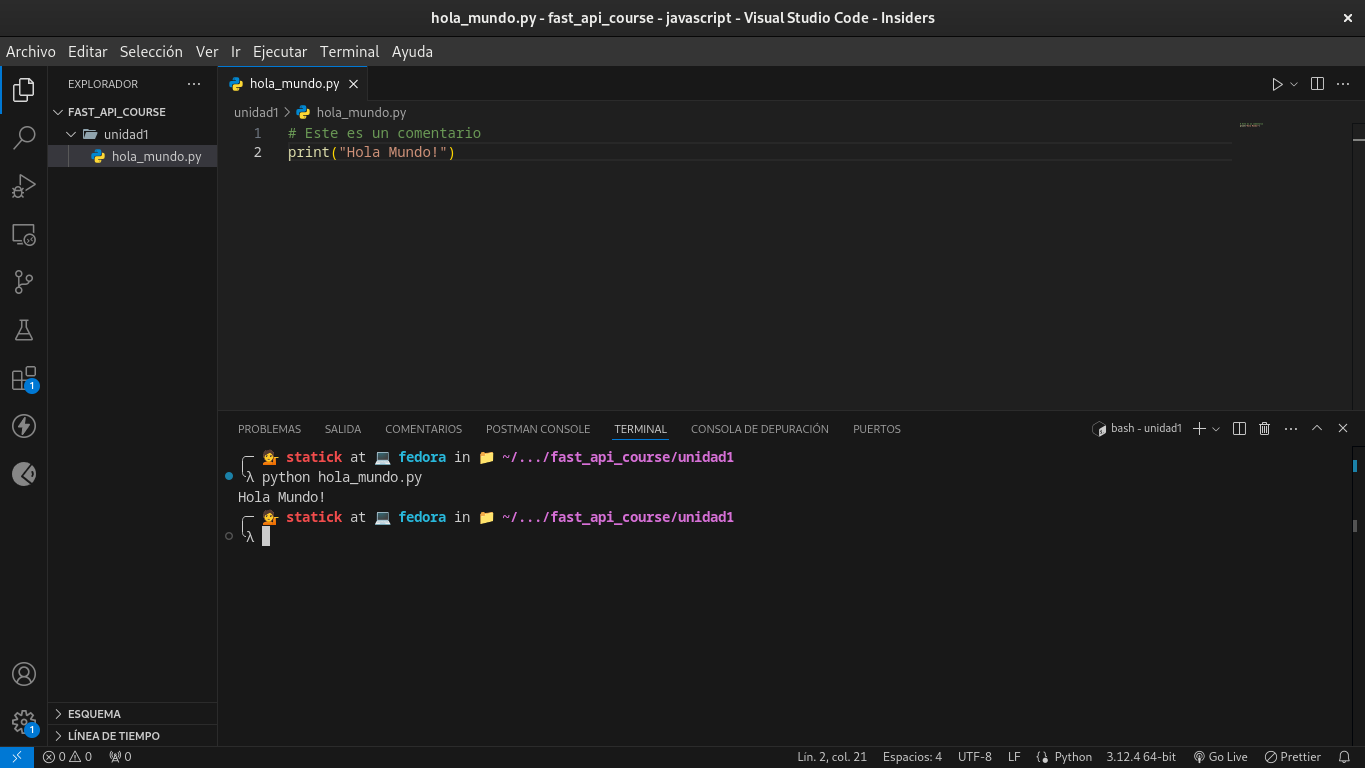
\includegraphics{unidades/unidad1/images/paste-2.png}

En este caso, el programa imprimirá en la terminal el mensaje
\textbf{Hola Mundo!}.

En este primer capítulo de la unidad, aprendimos la configuración básica
de python y la sintaxis básica para escribir programas en python.

\chapter{Variables y Control de
flujo}\label{variables-y-control-de-flujo}

\begin{figure}[H]

{\centering \includegraphics[width=2.08333in,height=\textheight]{index_files/mediabag/1200px-Python-logo-n.png}

}

\caption{Python}

\end{figure}%

En python las variables se pueden declarar sin necesidad de especificar
el tipo de dato, por lo que se puede asignar cualquier tipo de dato a
una variable, sin embargo en FastAPI es necesario especificar el tipo de
dato de las variables.

\begin{Shaded}
\begin{Highlighting}[]
\CommentTok{\# Declaración de variables}
\NormalTok{a }\OperatorTok{=} \DecValTok{5}
\NormalTok{b }\OperatorTok{=} \FloatTok{3.14}
\NormalTok{c }\OperatorTok{=} \StringTok{"Hola Mundo"}
\end{Highlighting}
\end{Shaded}

Para imprimir el valor de una variable se utiliza la función
\textbf{print()}.

\begin{Shaded}
\begin{Highlighting}[]
\BuiltInTok{print}\NormalTok{(a)}
\BuiltInTok{print}\NormalTok{(b)}
\BuiltInTok{print}\NormalTok{(c)}
\end{Highlighting}
\end{Shaded}

Para especìficar el tipo de dato de una variable se utiliza la siguiente
sintaxis:

\begin{Shaded}
\begin{Highlighting}[]
\CommentTok{\# Declaración de variables con tipo de dato}
\NormalTok{a: }\BuiltInTok{int} \OperatorTok{=} \DecValTok{5}
\NormalTok{b: }\BuiltInTok{float} \OperatorTok{=} \FloatTok{3.14}
\NormalTok{c: }\BuiltInTok{str} \OperatorTok{=} \StringTok{"Hola Mundo"}
\end{Highlighting}
\end{Shaded}

Para realizar operaciones aritméticas se utilizan los siguientes
operadores:

\begin{itemize}
\tightlist
\item
  Suma: +
\item
  Resta: -
\item
  Multiplicación: *
\item
  División: /
\item
  Módulo: \%
\item
  Exponente: **
\item
  División entera: //
\end{itemize}

\begin{Shaded}
\begin{Highlighting}[]
\CommentTok{\# Operaciones aritméticas}
\NormalTok{suma }\OperatorTok{=}\NormalTok{ a }\OperatorTok{+}\NormalTok{ b}
\NormalTok{resta }\OperatorTok{=}\NormalTok{ a }\OperatorTok{{-}}\NormalTok{ b}
\NormalTok{multiplicacion }\OperatorTok{=}\NormalTok{ a }\OperatorTok{*}\NormalTok{ b}
\NormalTok{division }\OperatorTok{=}\NormalTok{ a }\OperatorTok{/}\NormalTok{ b}
\NormalTok{modulo }\OperatorTok{=}\NormalTok{ a }\OperatorTok{\%}\NormalTok{ b}
\NormalTok{exponente }\OperatorTok{=}\NormalTok{ a }\OperatorTok{**}\NormalTok{ b}
\NormalTok{division\_entera }\OperatorTok{=}\NormalTok{ a }\OperatorTok{//}\NormalTok{ b}

\BuiltInTok{print}\NormalTok{(suma)}
\BuiltInTok{print}\NormalTok{(resta)}
\BuiltInTok{print}\NormalTok{(multiplicacion)}
\BuiltInTok{print}\NormalTok{(division)}
\BuiltInTok{print}\NormalTok{(modulo)}
\BuiltInTok{print}\NormalTok{(exponente)}
\BuiltInTok{print}\NormalTok{(division\_entera)}
\end{Highlighting}
\end{Shaded}

Para realizar comparaciones se utilizan los siguientes operadores:

\begin{itemize}
\tightlist
\item
  Igual que: ==
\item
  Diferente de: !=
\item
  Mayor que: \textgreater{}
\item
  Menor que: \textless{}
\item
  Mayor o igual que: \textgreater=
\item
  Menor o igual que: \textless=
\end{itemize}

\begin{Shaded}
\begin{Highlighting}[]
\CommentTok{\# Comparaciones}
\NormalTok{igual }\OperatorTok{=}\NormalTok{ a }\OperatorTok{==}\NormalTok{ b}
\NormalTok{diferente }\OperatorTok{=}
\end{Highlighting}
\end{Shaded}

Para realizar operaciones lógicas se utilizan los siguientes operadores:

\begin{itemize}
\tightlist
\item
  AND: and
\item
  OR: or
\item
  NOT: not
\end{itemize}

\begin{Shaded}
\begin{Highlighting}[]
\CommentTok{\# Operaciones lógicas}
\KeywordTok{and} \OperatorTok{=} \VariableTok{True} \KeywordTok{and} \VariableTok{False}
\KeywordTok{or} \OperatorTok{=} \VariableTok{True} \KeywordTok{or} \VariableTok{False}
\KeywordTok{not} \OperatorTok{=} \KeywordTok{not} \VariableTok{True}
\end{Highlighting}
\end{Shaded}

Para realizar estructuras de control de flujo se utilizan las siguientes
estructuras:

\begin{itemize}
\tightlist
\item
  if
\item
  elif
\item
  else
\end{itemize}

\begin{Shaded}
\begin{Highlighting}[]
\CommentTok{\# Estructuras de control de flujo}
\ControlFlowTok{if}\NormalTok{ a }\OperatorTok{\textgreater{}}\NormalTok{ b:}
    \BuiltInTok{print}\NormalTok{(}\StringTok{"a es mayor que b"}\NormalTok{)}
\ControlFlowTok{elif}\NormalTok{ a }\OperatorTok{\textless{}}\NormalTok{ b:}
    \BuiltInTok{print}\NormalTok{(}\StringTok{"a es menor que b"}\NormalTok{)}
\ControlFlowTok{else}\NormalTok{:}
    \BuiltInTok{print}\NormalTok{(}\StringTok{"a es igual a b"}\NormalTok{)}
\end{Highlighting}
\end{Shaded}

Tambien existen otras estructuras de control de flujo como:

\begin{itemize}
\tightlist
\item
  for
\item
  while
\end{itemize}

\begin{Shaded}
\begin{Highlighting}[]
\CommentTok{\# Estructuras de control de flujo}
\ControlFlowTok{for}\NormalTok{ i }\KeywordTok{in} \BuiltInTok{range}\NormalTok{(}\DecValTok{5}\NormalTok{):}
    \BuiltInTok{print}\NormalTok{(i)}
    
\NormalTok{i }\OperatorTok{=} \DecValTok{0}
\ControlFlowTok{while}\NormalTok{ i }\OperatorTok{\textless{}} \DecValTok{5}\NormalTok{:}
    \BuiltInTok{print}\NormalTok{(i)}
\NormalTok{    i }\OperatorTok{+=} \DecValTok{1}
\end{Highlighting}
\end{Shaded}

En FastAPI se pueden declarar variables en las rutas y se pueden
especificar el tipo de dato de las variables.

\begin{Shaded}
\begin{Highlighting}[]
\ImportTok{from}\NormalTok{ fastapi }\ImportTok{import}\NormalTok{ FastAPI}

\NormalTok{app }\OperatorTok{=}\NormalTok{ FastAPI()}

\AttributeTok{@app.get}\NormalTok{(}\StringTok{"/items/}\SpecialCharTok{\{item\_id\}}\StringTok{"}\NormalTok{)}
\ControlFlowTok{async} \KeywordTok{def}\NormalTok{ read\_item(item\_id: }\BuiltInTok{int}\NormalTok{):}
    \ControlFlowTok{return}\NormalTok{ \{}\StringTok{"item\_id"}\NormalTok{: item\_id\}}
\end{Highlighting}
\end{Shaded}

En el ejemplo anterior se declara una ruta con una variable llamada
\textbf{item\_id} de tipo entero, cuando analicemos FastAPI en sus
primeros capítulos se explicará con más detalle.

En este capítulo de la unidad, aprendimos a declarar variables, realizar
operaciones aritméticas, comparaciones, operaciones lógicas y
estructuras de control de flujo en python.

\chapter{Funciones y Parámetros}\label{funciones-y-paruxe1metros}

\begin{figure}[H]

{\centering \includegraphics[width=2.08333in,height=\textheight]{index_files/mediabag/1200px-Python-logo-n.png}

}

\caption{Python}

\end{figure}%

En Python las funciones se definen con la palabra clave \textbf{def}
seguida del nombre de la función y los parámetros entre paréntesis. A
continuación se muestra un ejemplo de una función que suma dos números:

\begin{Shaded}
\begin{Highlighting}[]
\KeywordTok{def}\NormalTok{ saludo():}
    \ControlFlowTok{return} \StringTok{"Hola Mundo!"}

\NormalTok{mensaje }\OperatorTok{=}\NormalTok{ saludo()}
\BuiltInTok{print}\NormalTok{(mensaje)}
\end{Highlighting}
\end{Shaded}

En el ejemplo anterior, la función \textbf{saludo()} retorna el mensaje
\textbf{Hola Mundo!}.

\section{Parámetros con valores por
defecto}\label{paruxe1metros-con-valores-por-defecto}

En Python es posible asignar valores por defecto a los parámetros de una
función. A continuación se muestra un ejemplo de una función que suma
dos números con un valor por defecto para el segundo parámetro:

\begin{Shaded}
\begin{Highlighting}[]
\KeywordTok{def}\NormalTok{ suma(a, b}\OperatorTok{=}\DecValTok{0}\NormalTok{):}
    \ControlFlowTok{return}\NormalTok{ a }\OperatorTok{+}\NormalTok{ b}

\NormalTok{resultado }\OperatorTok{=}\NormalTok{ suma(}\DecValTok{5}\NormalTok{)}
\BuiltInTok{print}\NormalTok{(resultado)}
\end{Highlighting}
\end{Shaded}

En el ejemplo anterior, la función \textbf{suma()} recibe dos
parámetros, el primer parámetro es obligatorio y el segundo parámetro
tiene un valor por defecto de \textbf{0}.

\section{Parámetros con nombre}\label{paruxe1metros-con-nombre}

En Python es posible pasar los parámetros de una función por nombre. A
continuación se muestra un ejemplo de una función que multiplica dos
números con los parámetros pasados por nombre:

\begin{Shaded}
\begin{Highlighting}[]
\KeywordTok{def}\NormalTok{ multiplicacion(a, b):}
    \ControlFlowTok{return}\NormalTok{ a }\OperatorTok{*}\NormalTok{ b}

\NormalTok{resultado }\OperatorTok{=}\NormalTok{ multiplicacion(b}\OperatorTok{=}\DecValTok{5}\NormalTok{, a}\OperatorTok{=}\DecValTok{3}\NormalTok{)}
\BuiltInTok{print}\NormalTok{(resultado)}
\end{Highlighting}
\end{Shaded}

En el ejemplo anterior, los parámetros de la función
\textbf{multiplicacion()} se pasan por nombre, por lo que el orden de
los parámetros no importa.

\begin{tcolorbox}[enhanced jigsaw, toprule=.15mm, title=\textcolor{quarto-callout-tip-color}{\faLightbulb}\hspace{0.5em}{Tip}, opacitybacktitle=0.6, colbacktitle=quarto-callout-tip-color!10!white, toptitle=1mm, breakable, left=2mm, coltitle=black, colback=white, bottomrule=.15mm, colframe=quarto-callout-tip-color-frame, bottomtitle=1mm, arc=.35mm, titlerule=0mm, opacityback=0, rightrule=.15mm, leftrule=.75mm]

Cuando aprendamos acerca de la POO (Programaciòn Orientada a Objetos)
veremos que las \textbf{funciones} que se definen dentro de una clase se
llaman \textbf{métodos}.

\end{tcolorbox}

En FastAPI es posible definir funciones que se ejecutan cuando se
realiza una petición HTTP a una ruta específica. Cuando analicemos
FastAPI veremos cómo definir funciones que se ejecutan cuando se realiza
una petición HTTP a una ruta específica.

En este tercer capítulo de la unidad, aprendimos a definir funciones en
Python y a utilizar parámetros con valores por defecto y parámetros con
nombre.

\part{Unidad 2: Estructura de Datos en Python}

\chapter{Listas y Tuplas}\label{listas-y-tuplas}

\begin{figure}[H]

{\centering \includegraphics[width=2.08333in,height=\textheight]{index_files/mediabag/1200px-Python-logo-n.png}

}

\caption{Python}

\end{figure}%

En este capículo de la segunda unidad vamos a aprender acerca de las
listas y las tuplas en Python.

En Python, las listas y las tuplas son estructuras de datos que permiten
almacenar múltiples elementos en una sola variable.

\section{Listas}\label{listas}

Las listas en Python se definen utilizando corchetes \textbf{{[} {]}} y
los elementos de la lista se separan por comas \textbf{,}. A
continuación se muestra un ejemplo de una lista con números enteros:

\begin{Shaded}
\begin{Highlighting}[]
\CommentTok{\# Declaración de una lista}
\NormalTok{numeros }\OperatorTok{=}\NormalTok{ [}\DecValTok{1}\NormalTok{, }\DecValTok{2}\NormalTok{, }\DecValTok{3}\NormalTok{, }\DecValTok{4}\NormalTok{, }\DecValTok{5}\NormalTok{]}
\end{Highlighting}
\end{Shaded}

Para acceder a un elemento de la lista se utiliza el índice del
elemento. Los índices en Python empiezan en \textbf{0}. A continuación
se muestra un ejemplo de cómo acceder al primer elemento de la lista:

\begin{Shaded}
\begin{Highlighting}[]
\CommentTok{\# Acceso a un elemento de la lista}
\NormalTok{primer\_elemento }\OperatorTok{=}\NormalTok{ numeros[}\DecValTok{0}\NormalTok{]}
\BuiltInTok{print}\NormalTok{(primer\_elemento)}
\end{Highlighting}
\end{Shaded}

Para agregar un elemento a la lista se utiliza el método
\textbf{append()}. A continuación se muestra un ejemplo de cómo agregar
un elemento a la lista:

\begin{Shaded}
\begin{Highlighting}[]
\CommentTok{\# Agregar un elemento a la lista}
\NormalTok{numeros.append(}\DecValTok{6}\NormalTok{)}
\BuiltInTok{print}\NormalTok{(numeros)}
\end{Highlighting}
\end{Shaded}

Para eliminar un elemento de la lista se utiliza el método
\textbf{remove()}. A continuación se muestra un ejemplo de cómo eliminar
un elemento de la lista:

\begin{Shaded}
\begin{Highlighting}[]
\CommentTok{\# Eliminar un elemento de la lista}
\NormalTok{numeros.remove(}\DecValTok{3}\NormalTok{)}
\BuiltInTok{print}\NormalTok{(numeros)}
\end{Highlighting}
\end{Shaded}

\section{Tuplas}\label{tuplas}

Las tuplas en Python se definen utilizando paréntesis \textbf{( )} y los
elementos de la tupla se separan por comas \textbf{,}. A continuación se
muestra un ejemplo de una tupla con números enteros:

\begin{Shaded}
\begin{Highlighting}[]
\CommentTok{\# Declaración de una tupla}
\NormalTok{numeros }\OperatorTok{=}\NormalTok{ (}\DecValTok{1}\NormalTok{, }\DecValTok{2}\NormalTok{, }\DecValTok{3}\NormalTok{, }\DecValTok{4}\NormalTok{, }\DecValTok{5}\NormalTok{)}
\end{Highlighting}
\end{Shaded}

Para acceder a un elemento de la tupla se utiliza el índice del
elemento. Los índices en Python empiezan en \textbf{0}. A continuación
se muestra un ejemplo de cómo acceder al primer elemento de la tupla:

\begin{Shaded}
\begin{Highlighting}[]
\CommentTok{\# Acceso a un elemento de la tupla}
\NormalTok{primer\_elemento }\OperatorTok{=}\NormalTok{ numeros[}\DecValTok{0}\NormalTok{]}
\BuiltInTok{print}\NormalTok{(primer\_elemento)}
\end{Highlighting}
\end{Shaded}

Las tuplas son inmutables, lo que significa que una vez que se crea una
tupla no se pueden modificar los elementos de la tupla. A continuación
se muestra un ejemplo de cómo intentar modificar un elemento de la
tupla:

\begin{Shaded}
\begin{Highlighting}[]
\CommentTok{\# Intentar modificar un elemento de la tupla}
\NormalTok{numeros[}\DecValTok{0}\NormalTok{] }\OperatorTok{=} \DecValTok{10}
\end{Highlighting}
\end{Shaded}

En FastAPI es posible utilizar listas y tuplas para definir los
parámetros de una función. Cuando analicemos FastAPI veremos cómo
utilizar listas y tuplas para definir los parámetros de una función.

En este capítulo de la unidad, aprendimos acerca de las listas y las
tuplas en Python.

\chapter{Diccionarios y Conjuntos}\label{diccionarios-y-conjuntos}

\begin{figure}[H]

{\centering \includegraphics[width=2.08333in,height=\textheight]{index_files/mediabag/1200px-Python-logo-n.png}

}

\caption{Python}

\end{figure}%

En este capítulo vamos a aprender acerca de los diccionarios y los
conjuntos en Python.

\section{Diccionarios}\label{diccionarios}

Los diccionarios en Python son estructuras de datos que permiten
almacenar pares clave-valor en una sola variable. Los diccionarios se
definen utilizando llaves \textbf{\{ \}} y los pares clave-valor se
separan por comas \textbf{,}. A continuación se muestra un ejemplo de un
diccionario con nombres de personas y sus edades:

\begin{Shaded}
\begin{Highlighting}[]
\CommentTok{\# Declaración de un diccionario}

\NormalTok{personas }\OperatorTok{=}\NormalTok{ \{}
    \StringTok{"Juan"}\NormalTok{: }\DecValTok{25}\NormalTok{,}
    \StringTok{"Maria"}\NormalTok{: }\DecValTok{30}\NormalTok{,}
    \StringTok{"Pedro"}\NormalTok{: }\DecValTok{35}
\NormalTok{\}}
\end{Highlighting}
\end{Shaded}

Para acceder a un valor del diccionario se utiliza la clave del valor. A
continuación se muestra un ejemplo de cómo acceder a la edad de la
persona \textbf{Juan}:

\begin{Shaded}
\begin{Highlighting}[]
\CommentTok{\# Acceso a un valor del diccionario}

\NormalTok{edad\_juan }\OperatorTok{=}\NormalTok{ personas[}\StringTok{"Juan"}\NormalTok{]}
\BuiltInTok{print}\NormalTok{(edad\_juan)}
\end{Highlighting}
\end{Shaded}

Para agregar un par clave-valor al diccionario se utiliza la siguiente
sintaxis:

\begin{Shaded}
\begin{Highlighting}[]
\CommentTok{\# Agregar un par clave{-}valor al diccionario}

\NormalTok{personas[}\StringTok{"Ana"}\NormalTok{] }\OperatorTok{=} \DecValTok{40}
\BuiltInTok{print}\NormalTok{(personas)}
\end{Highlighting}
\end{Shaded}

Para eliminar un par clave-valor del diccionario se utiliza la siguiente
sintaxis:

\begin{Shaded}
\begin{Highlighting}[]
\CommentTok{\# Eliminar un par clave{-}valor del diccionario}

\KeywordTok{del}\NormalTok{ personas[}\StringTok{"Pedro"}\NormalTok{]}
\BuiltInTok{print}\NormalTok{(personas)}
\end{Highlighting}
\end{Shaded}

\section{Conjuntos}\label{conjuntos}

Los conjuntos en Python son estructuras de datos que permiten almacenar
elementos únicos en una sola variable. Los conjuntos se definen
utilizando llaves \textbf{\{ \}} y los elementos del conjunto se separan
por comas \textbf{,}. A continuación se muestra un ejemplo de un
conjunto con números enteros:

\begin{Shaded}
\begin{Highlighting}[]
\CommentTok{\# Declaración de un conjunto}

\NormalTok{numeros }\OperatorTok{=}\NormalTok{ \{}\DecValTok{1}\NormalTok{, }\DecValTok{2}\NormalTok{, }\DecValTok{3}\NormalTok{, }\DecValTok{4}\NormalTok{, }\DecValTok{5}\NormalTok{\}}
\end{Highlighting}
\end{Shaded}

Para agregar un elemento al conjunto se utiliza el método
\textbf{add()}. A continuación se muestra un ejemplo de cómo agregar un
elemento al conjunto:

\begin{Shaded}
\begin{Highlighting}[]
\CommentTok{\# Agregar un elemento al conjunto}

\NormalTok{numeros.add(}\DecValTok{6}\NormalTok{)}
\BuiltInTok{print}\NormalTok{(numeros)}
\end{Highlighting}
\end{Shaded}

Para eliminar un elemento del conjunto se utiliza el método
\textbf{remove()}. A continuación se muestra un ejemplo de cómo eliminar
un elemento del conjunto:

\begin{Shaded}
\begin{Highlighting}[]
\CommentTok{\# Eliminar un elemento del conjunto}

\NormalTok{numeros.remove(}\DecValTok{3}\NormalTok{)}
\BuiltInTok{print}\NormalTok{(numeros)}
\end{Highlighting}
\end{Shaded}

En FastAPI es posible utilizar diccionarios y conjuntos para almacenar
información y realizar operaciones con ellos. Cuando analicemos FastAPI
veremos cómo utilizar diccionarios y conjuntos para almacenar
información y realizar operaciones con ellos.

En este capítulo aprendimos acerca de los diccionarios y los conjuntos
en Python.

\part{Unidad 3: Programación Orientada a Objetos en Python}

\chapter{Conceptos Básicos}\label{conceptos-buxe1sicos}

\begin{figure}[H]

{\centering \includegraphics[width=2.08333in,height=\textheight]{index_files/mediabag/1200px-Python-logo-n.png}

}

\caption{Python}

\end{figure}%

En este capítulo vamos a aprender acerca de los conceptos básicos de la
Programación Orientada a Objetos (POO) en Python.

\section{Clases y Objetos}\label{clases-y-objetos}

En la Programación Orientada a Objetos (POO) los objetos son instancias
de clases. Las clases son plantillas que definen las propiedades y los
métodos de los objetos. A continuación se muestra un ejemplo de una
clase en Python:

\begin{Shaded}
\begin{Highlighting}[]
\CommentTok{\# Declaración de una clase}

\KeywordTok{class}\NormalTok{ Persona:}
    \KeywordTok{def} \FunctionTok{\_\_init\_\_}\NormalTok{(}\VariableTok{self}\NormalTok{, nombre, edad):}
        \VariableTok{self}\NormalTok{.nombre }\OperatorTok{=}\NormalTok{ nombre}
        \VariableTok{self}\NormalTok{.edad }\OperatorTok{=}\NormalTok{ edad}

    \KeywordTok{def}\NormalTok{ saludar(}\VariableTok{self}\NormalTok{):}
        \ControlFlowTok{return} \SpecialStringTok{f"Hola, mi nombre es }\SpecialCharTok{\{}\VariableTok{self}\SpecialCharTok{.}\NormalTok{nombre}\SpecialCharTok{\}}\SpecialStringTok{ y tengo }\SpecialCharTok{\{}\VariableTok{self}\SpecialCharTok{.}\NormalTok{edad}\SpecialCharTok{\}}\SpecialStringTok{ años."}
\end{Highlighting}
\end{Shaded}

En el ejemplo anterior se declara una clase llamada \textbf{Persona} con
dos propiedades \textbf{nombre} y \textbf{edad} y un método
\textbf{saludar()} que retorna un mensaje con el nombre y la edad de la
persona.

Para crear un objeto de la clase \textbf{Persona} se utiliza la
siguiente sintaxis:

\begin{Shaded}
\begin{Highlighting}[]
\CommentTok{\# Creación de un objeto de la clase Persona}

\NormalTok{persona }\OperatorTok{=}\NormalTok{ Persona(}\StringTok{"Juan"}\NormalTok{, }\DecValTok{25}\NormalTok{)}
\NormalTok{mensaje }\OperatorTok{=}\NormalTok{ persona.saludar()}
\BuiltInTok{print}\NormalTok{(mensaje)}
\end{Highlighting}
\end{Shaded}

En el ejemplo anterior se crea un objeto de la clase \textbf{Persona}
con el nombre \textbf{Juan} y la edad \textbf{25} y se llama al método
\textbf{saludar()} del objeto \textbf{persona}.

En FastAPI es posible definir clases que se utilizan para definir los
modelos de los datos que se envían y reciben en las peticiones HTTP.
Cuando analicemos FastAPI veremos cómo definir clases que se utilizan
para definir los modelos de los datos que se envían y reciben en las
peticiones HTTP.

En este capítulo de la unidad, aprendimos acerca de las clases y los
objetos en la Programación Orientada a Objetos (POO) en Python.

\chapter{Herencia, Polimorfismo y
Encapsulación}\label{herencia-polimorfismo-y-encapsulaciuxf3n}

\begin{figure}[H]

{\centering \includegraphics[width=2.08333in,height=\textheight]{index_files/mediabag/1200px-Python-logo-n.png}

}

\caption{Python}

\end{figure}%

En este capítulo vamos a aprender acerca de la herencia y el
polimorfismo en la Programación Orientada a Objetos (POO) en Python.

\section{Herencia}\label{herencia}

La herencia en la Programación Orientada a Objetos (POO) es un mecanismo
que permite crear una nueva clase a partir de una clase existente. La
nueva clase hereda las propiedades y los métodos de la clase existente.
A continuación se muestra un ejemplo de una clase \textbf{Vehiculo} con
las propiedades \textbf{marca} y \textbf{modelo} y un método
\textbf{mostrar()} que retorna un mensaje con la marca y el modelo del
vehículo:

\begin{Shaded}
\begin{Highlighting}[]
\CommentTok{\# Declaración de una clase Vehiculo}

\KeywordTok{class}\NormalTok{ Vehiculo:}
    \KeywordTok{def} \FunctionTok{\_\_init\_\_}\NormalTok{(}\VariableTok{self}\NormalTok{, marca, modelo):}
        \VariableTok{self}\NormalTok{.marca }\OperatorTok{=}\NormalTok{ marca}
        \VariableTok{self}\NormalTok{.modelo }\OperatorTok{=}\NormalTok{ modelo}

    \KeywordTok{def}\NormalTok{ mostrar(}\VariableTok{self}\NormalTok{):}
        \ControlFlowTok{return} \SpecialStringTok{f"Vehículo: }\SpecialCharTok{\{}\VariableTok{self}\SpecialCharTok{.}\NormalTok{marca}\SpecialCharTok{\}}\SpecialStringTok{ }\SpecialCharTok{\{}\VariableTok{self}\SpecialCharTok{.}\NormalTok{modelo}\SpecialCharTok{\}}\SpecialStringTok{"}
\end{Highlighting}
\end{Shaded}

En el ejemplo anterior se declara una clase \textbf{Vehiculo} con las
propiedades \textbf{marca} y \textbf{modelo} y un método
\textbf{mostrar()} que retorna un mensaje con la marca y el modelo del
vehículo.

Para crear una nueva clase \textbf{Auto} que hereda de la clase
\textbf{Vehiculo} se utiliza la siguiente sintaxis:

\begin{Shaded}
\begin{Highlighting}[]
\CommentTok{\# Declaración de una clase Auto que hereda de la clase Vehiculo}

\KeywordTok{class}\NormalTok{ Auto(Vehiculo):}
    \KeywordTok{def} \FunctionTok{\_\_init\_\_}\NormalTok{(}\VariableTok{self}\NormalTok{, marca, modelo, color):}
        \BuiltInTok{super}\NormalTok{().}\FunctionTok{\_\_init\_\_}\NormalTok{(marca, modelo)}
        \VariableTok{self}\NormalTok{.color }\OperatorTok{=}\NormalTok{ color}

    \KeywordTok{def}\NormalTok{ mostrar(}\VariableTok{self}\NormalTok{):}
        \ControlFlowTok{return} \SpecialStringTok{f"Auto: }\SpecialCharTok{\{}\VariableTok{self}\SpecialCharTok{.}\NormalTok{marca}\SpecialCharTok{\}}\SpecialStringTok{ }\SpecialCharTok{\{}\VariableTok{self}\SpecialCharTok{.}\NormalTok{modelo}\SpecialCharTok{\}}\SpecialStringTok{ de color }\SpecialCharTok{\{}\VariableTok{self}\SpecialCharTok{.}\NormalTok{color}\SpecialCharTok{\}}\SpecialStringTok{"}
\end{Highlighting}
\end{Shaded}

En el ejemplo anterior se declara una clase \textbf{Auto} que hereda de
la clase \textbf{Vehiculo} con la propiedad \textbf{color} y un método
\textbf{mostrar()} que retorna un mensaje con la marca, el modelo y el
color del auto.

Para crear un objeto de la clase \textbf{Auto} se utiliza la siguiente
sintaxis:

\begin{Shaded}
\begin{Highlighting}[]
\CommentTok{\# Creación de un objeto de la clase Auto}

\NormalTok{auto }\OperatorTok{=}\NormalTok{ Auto(}\StringTok{"Toyota"}\NormalTok{, }\StringTok{"Corolla"}\NormalTok{, }\StringTok{"Rojo"}\NormalTok{)}
\NormalTok{mensaje }\OperatorTok{=}\NormalTok{ auto.mostrar()}
\BuiltInTok{print}\NormalTok{(mensaje)}
\end{Highlighting}
\end{Shaded}

En el ejemplo anterior se crea un objeto de la clase \textbf{Auto} con
la marca \textbf{Toyota}, el modelo \textbf{Corolla} y el color
\textbf{Rojo} y se llama al método \textbf{mostrar()} del objeto
\textbf{auto}.

\section{Polimorfismo}\label{polimorfismo}

El polimorfismo en la Programación Orientada a Objetos (POO) es un
mecanismo que permite que un objeto se com

\begin{Shaded}
\begin{Highlighting}[]
\CommentTok{\# Declaración de una clase Vehiculo}

\KeywordTok{class}\NormalTok{ Vehiculo:}
    \KeywordTok{def} \FunctionTok{\_\_init\_\_}\NormalTok{(}\VariableTok{self}\NormalTok{, marca, modelo):}
        \VariableTok{self}\NormalTok{.marca }\OperatorTok{=}\NormalTok{ marca}
        \VariableTok{self}\NormalTok{.modelo }\OperatorTok{=}\NormalTok{ modelo}

    \KeywordTok{def}\NormalTok{ mostrar(}\VariableTok{self}\NormalTok{):}
        \ControlFlowTok{return} \SpecialStringTok{f"Vehículo: }\SpecialCharTok{\{}\VariableTok{self}\SpecialCharTok{.}\NormalTok{marca}\SpecialCharTok{\}}\SpecialStringTok{ }\SpecialCharTok{\{}\VariableTok{self}\SpecialCharTok{.}\NormalTok{modelo}\SpecialCharTok{\}}\SpecialStringTok{"}
\end{Highlighting}
\end{Shaded}

En el ejemplo anterior se declara una clase \textbf{Vehiculo} con las
propiedades \textbf{marca} y \textbf{modelo} y un método
\textbf{mostrar()} que retorna un mensaje con la marca y el modelo del
vehículo.

Para crear una nueva clase \textbf{Auto} que hereda de la clase
\textbf{Vehiculo} se utiliza la siguiente sintaxis:

\begin{Shaded}
\begin{Highlighting}[]
\CommentTok{\# Declaración de una clase Auto que hereda de la clase Vehiculo}

\KeywordTok{class}\NormalTok{ Auto(Vehiculo):}
    \KeywordTok{def} \FunctionTok{\_\_init\_\_}\NormalTok{(}\VariableTok{self}\NormalTok{, marca, modelo, color):}
        \BuiltInTok{super}\NormalTok{().}\FunctionTok{\_\_init\_\_}\NormalTok{(marca, modelo)}
        \VariableTok{self}\NormalTok{.color }\OperatorTok{=}\NormalTok{ color}

    \KeywordTok{def}\NormalTok{ mostrar(}\VariableTok{self}\NormalTok{):}
        \ControlFlowTok{return} \SpecialStringTok{f"Auto: }\SpecialCharTok{\{}\VariableTok{self}\SpecialCharTok{.}\NormalTok{marca}\SpecialCharTok{\}}\SpecialStringTok{ }\SpecialCharTok{\{}\VariableTok{self}\SpecialCharTok{.}\NormalTok{modelo}\SpecialCharTok{\}}\SpecialStringTok{ de color }\SpecialCharTok{\{}\VariableTok{self}\SpecialCharTok{.}\NormalTok{color}\SpecialCharTok{\}}\SpecialStringTok{"}
\end{Highlighting}
\end{Shaded}

En el ejemplo anterior se declara una clase \textbf{Auto} que hereda de
la clase \textbf{Vehiculo} con la propiedad \textbf{color} y un método
\textbf{mostrar()} que retorna un mensaje con la marca, el modelo y el
color del auto.

Para crear un objeto de la clase \textbf{Auto} se utiliza la siguiente
sintaxis:

\begin{Shaded}
\begin{Highlighting}[]
\CommentTok{\# Creación de un objeto de la clase Auto}

\NormalTok{auto }\OperatorTok{=}\NormalTok{ Auto(}\StringTok{"Toyota"}\NormalTok{, }\StringTok{"Corolla"}\NormalTok{, }\StringTok{"Rojo"}\NormalTok{)}
\NormalTok{mensaje }\OperatorTok{=}\NormalTok{ auto.mostrar()}
\BuiltInTok{print}\NormalTok{(mensaje)}
\end{Highlighting}
\end{Shaded}

En el ejemplo anterior se crea un objeto de la clase \textbf{Auto} con
la marca \textbf{Toyota}, el modelo \textbf{Corolla} y el color
\textbf{Rojo} y se llama al método \textbf{mostrar()} del objeto
\textbf{auto}.

\section{Encapsulamiento}\label{encapsulamiento}

El encapsulamiento en la Programación Orientada a Objetos (POO) es un
mecanismo que permite ocultar los detalles de implementación de una
clase y exponer solo la interfaz de la clase. En Python, el
encapsulamiento se logra utilizando los siguientes modificadores de
acceso:

\begin{itemize}
\item
  \textbf{Público}: Los miembros de la clase son públicos y se pueden
  acceder desde cualquier parte del programa.
\item
  \textbf{Protegido}: Los miembros de la clase son protegidos y se
  pueden acceder desde la clase y las clases derivadas.
\item
  \textbf{Privado}: Los miembros de la clase son privados y solo se
  pueden acceder desde la clase.
\end{itemize}

A continuación se muestra un ejemplo de una clase \textbf{Persona} con
los modificadores de acceso \textbf{público}, \textbf{protegido} y
\textbf{privado}:

\begin{Shaded}
\begin{Highlighting}[]
\CommentTok{\# Declaración de una clase Persona}

\KeywordTok{class}\NormalTok{ Persona:}
    \KeywordTok{def} \FunctionTok{\_\_init\_\_}\NormalTok{(}\VariableTok{self}\NormalTok{, nombre, edad):}
        \VariableTok{self}\NormalTok{.nombre }\OperatorTok{=}\NormalTok{ nombre}
        \VariableTok{self}\NormalTok{.\_edad }\OperatorTok{=}\NormalTok{ edad}
        \VariableTok{self}\NormalTok{.\_\_dni }\OperatorTok{=} \StringTok{"12345678"}

    \KeywordTok{def}\NormalTok{ mostrar(}\VariableTok{self}\NormalTok{):}
        \ControlFlowTok{return} \SpecialStringTok{f"Persona: }\SpecialCharTok{\{}\VariableTok{self}\SpecialCharTok{.}\NormalTok{nombre}\SpecialCharTok{\}}\SpecialStringTok{ }\SpecialCharTok{\{}\VariableTok{self}\SpecialCharTok{.}\NormalTok{\_edad}\SpecialCharTok{\}}\SpecialStringTok{ }\SpecialCharTok{\{}\VariableTok{self}\SpecialCharTok{.}\NormalTok{\_\_dni}\SpecialCharTok{\}}\SpecialStringTok{"}

\CommentTok{\# Creación de un objeto de la clase Persona}

\NormalTok{persona }\OperatorTok{=}\NormalTok{ Persona(}\StringTok{"Juan"}\NormalTok{, }\DecValTok{25}\NormalTok{)}
\NormalTok{mensaje }\OperatorTok{=}\NormalTok{ persona.mostrar()}
\BuiltInTok{print}\NormalTok{(mensaje)}
\end{Highlighting}
\end{Shaded}

En el ejemplo anterior se declara una clase \textbf{Persona} con los
modificadores de acceso \textbf{público}, \textbf{protegido} y
\textbf{privado} y se crea un objeto de la clase \textbf{Persona} con el
nombre \textbf{Juan}, la edad \textbf{25} y el DNI \textbf{12345678}.

En FastAPI es posible definir clases que se utilizan para definir los
modelos de los datos que se envían y reciben en las peticiones HTTP.
Cuando analicemos FastAPI veremos cómo definir clases que se utilizan
para definir los modelos de los datos que se envían y reciben en las
peticiones HTTP.

En este capítulo de la unidad, aprendimos acerca de la herencia,
polimorfismo y encapsulación en la Programación Orientada a Objetos
(POO) en Python.

\part{Unidad 4: Herramientas de Desarrollo}

\chapter{Git y Github}\label{git-y-github}

\includegraphics[width=2.08333in,height=\textheight]{index_files/mediabag/1280px-Git-logo.svg.png}
\includegraphics[width=1.5625in,height=\textheight]{index_files/mediabag/1024px-Octicons-mark.png}

En este capítulo un poco diferente vamos a aprender acerca de
\textbf{Git} y \textbf{Github}. Sin embargo lo aplicaremos con el
leguaje de programación \textbf{Python}.

\section{Git}\label{git}

\begin{figure}[H]

{\centering \includegraphics[width=2.08333in,height=\textheight]{index_files/mediabag/1280px-Git-logo.svg.png}

}

\caption{Git}

\end{figure}%

\textbf{Git} es un sistema de control de versiones distribuido que
permite llevar un registro de los cambios en los archivos de un
proyecto. \textbf{Git} es ampliamente utilizado en el desarrollo de
software para colaborar en proyectos con otros desarrolladores.

\subsection{Instalación de Git}\label{instalaciuxf3n-de-git}

Para instalar \textbf{Git} en tu computadora, sigue los siguientes
pasos:

\begin{enumerate}
\def\labelenumi{\arabic{enumi}.}
\item
  Descarga el instalador de \textbf{Git} desde el siguiente enlace:
  \url{https://git-scm.com/}.
\item
  Ejecuta el instalador de \textbf{Git} y sigue las instrucciones del
  instalador.
\item
  Verifica que \textbf{Git} se ha instalado correctamente ejecutando el
  siguiente comando en la terminal:
\end{enumerate}

\begin{Shaded}
\begin{Highlighting}[]
\FunctionTok{git} \AttributeTok{{-}{-}version}
\end{Highlighting}
\end{Shaded}

Si \textbf{Git} se ha instalado correctamente, verás un mensaje similar
a este:

\begin{Shaded}
\begin{Highlighting}[]
\FunctionTok{git}\NormalTok{ version 2.45.2}
\end{Highlighting}
\end{Shaded}

\subsection{Comandos básicos de Git}\label{comandos-buxe1sicos-de-git}

A continuación se muestran algunos comandos básicos de \textbf{Git} que
te serán útiles para trabajar con \textbf{Git}:

\begin{itemize}
\tightlist
\item
  \textbf{git init}: Inicializa un repositorio de \textbf{Git} en el
  directorio actual.
\end{itemize}

\begin{Shaded}
\begin{Highlighting}[]
\FunctionTok{git}\NormalTok{ init}
\end{Highlighting}
\end{Shaded}

\begin{itemize}
\tightlist
\item
  \textbf{git add}: Agrega los archivos al área de preparación.
\end{itemize}

\begin{Shaded}
\begin{Highlighting}[]
\FunctionTok{git}\NormalTok{ add archivo.py}
\end{Highlighting}
\end{Shaded}

\begin{itemize}
\tightlist
\item
  \textbf{git commit}: Guarda los cambios en el repositorio.
\end{itemize}

\begin{Shaded}
\begin{Highlighting}[]
\FunctionTok{git}\NormalTok{ commit }\AttributeTok{{-}m} \StringTok{"Mensaje del commit"}
\end{Highlighting}
\end{Shaded}

\begin{itemize}
\tightlist
\item
  \textbf{git status}: Muestra el estado de los archivos en el
  repositorio.
\end{itemize}

\begin{Shaded}
\begin{Highlighting}[]
\FunctionTok{git}\NormalTok{ status}
\end{Highlighting}
\end{Shaded}

\begin{itemize}
\tightlist
\item
  \textbf{git log}: Muestra el historial de los commits en el
  repositorio.
\end{itemize}

\begin{Shaded}
\begin{Highlighting}[]
\FunctionTok{git}\NormalTok{ log}
\end{Highlighting}
\end{Shaded}

\section{Github}\label{github}

\begin{figure}[H]

{\centering \includegraphics[width=1.5625in,height=\textheight]{index_files/mediabag/1024px-Octicons-mark.png}

}

\caption{Github}

\end{figure}%

\textbf{Github} es una plataforma en línea que permite alojar proyectos
de \textbf{Git} de forma gratuita. \textbf{Github} es ampliamente
utilizado en el desarrollo de software para colaborar en proyectos con
otros desarrolladores.

\subsection{Crear una cuenta en
Github}\label{crear-una-cuenta-en-github}

Para crear una cuenta en \textbf{Github}, sigue los siguientes pasos:

\begin{enumerate}
\def\labelenumi{\arabic{enumi}.}
\item
  Ingresa a la página de \textbf{Github}: \url{https://github.com}.
\item
  Haz clic en el botón \textbf{Sign up}.
\item
  Completa el formulario de registro con tu nombre de usuario, dirección
  de correo electrónico y contraseña.
\item
  Haz clic en el botón \textbf{Create account}.
\item
  Verifica tu dirección de correo electrónico.
\end{enumerate}

\subsection{Crear un repositorio en
Github}\label{crear-un-repositorio-en-github}

Para crear un repositorio en \textbf{Github}, sigue los siguientes
pasos:

\begin{enumerate}
\def\labelenumi{\arabic{enumi}.}
\item
  Inicia sesión en tu cuenta de \textbf{Github}.
\item
  Haz clic en el botón \textbf{New}.
\item
  Completa el formulario con el nombre del repositorio, la descripción y
  la visibilidad del repositorio.
\item
  Haz clic en el botón \textbf{Create repository}.
\item
  Copia la URL del repositorio.
\end{enumerate}

\subsection{Clonar un repositorio en
Github}\label{clonar-un-repositorio-en-github}

Para clonar un repositorio en \textbf{Github}, sigue los siguientes
pasos:

\begin{enumerate}
\def\labelenumi{\arabic{enumi}.}
\item
  Copia la URL del repositorio.
\item
  Abre la terminal y ejecuta el siguiente comando:
\end{enumerate}

\begin{Shaded}
\begin{Highlighting}[]
\FunctionTok{git}\NormalTok{ clone URL\_del\_repositorio}
\end{Highlighting}
\end{Shaded}

\begin{enumerate}
\def\labelenumi{\arabic{enumi}.}
\setcounter{enumi}{2}
\item
  Ingresa tus credenciales de \textbf{Github}.
\item
  El repositorio se clonará en tu computadora.
\end{enumerate}

\subsection{Subir cambios a un repositorio en
Github}\label{subir-cambios-a-un-repositorio-en-github}

Para subir cambios a un repositorio en \textbf{Github}, sigue los
siguientes pasos:

\begin{enumerate}
\def\labelenumi{\arabic{enumi}.}
\tightlist
\item
  Agrega los archivos al área de preparación.
\end{enumerate}

\begin{Shaded}
\begin{Highlighting}[]
\FunctionTok{git}\NormalTok{ add archivo.py}
\end{Highlighting}
\end{Shaded}

\begin{enumerate}
\def\labelenumi{\arabic{enumi}.}
\setcounter{enumi}{1}
\tightlist
\item
  Guarda los cambios en el repositorio.
\end{enumerate}

\begin{Shaded}
\begin{Highlighting}[]
\FunctionTok{git}\NormalTok{ commit }\AttributeTok{{-}m} \StringTok{"Mensaje del commit"}
\end{Highlighting}
\end{Shaded}

\begin{enumerate}
\def\labelenumi{\arabic{enumi}.}
\setcounter{enumi}{2}
\tightlist
\item
  Sube los cambios al repositorio en \textbf{Github}.
\end{enumerate}

\begin{Shaded}
\begin{Highlighting}[]
\FunctionTok{git}\NormalTok{ push}
\end{Highlighting}
\end{Shaded}

\begin{enumerate}
\def\labelenumi{\arabic{enumi}.}
\setcounter{enumi}{3}
\item
  Ingresa tus credenciales de \textbf{Github}.
\item
  Los cambios se subirán al repositorio en \textbf{Github}.
\end{enumerate}

\subsection{Descargar cambios de un repositorio en
Github}\label{descargar-cambios-de-un-repositorio-en-github}

Para descargar cambios de un repositorio en \textbf{Github}, sigue los
siguientes pasos:

\begin{enumerate}
\def\labelenumi{\arabic{enumi}.}
\tightlist
\item
  Descarga los cambios del repositorio en \textbf{Github}.
\end{enumerate}

\begin{Shaded}
\begin{Highlighting}[]
\FunctionTok{git}\NormalTok{ pull}
\end{Highlighting}
\end{Shaded}

\begin{enumerate}
\def\labelenumi{\arabic{enumi}.}
\setcounter{enumi}{1}
\item
  Ingresa tus credenciales de \textbf{Github}.
\item
  Los cambios se descargarán del repositorio en \textbf{Github}.
\end{enumerate}

En FastAPI es posible utilizar \textbf{Git} y \textbf{Github} para
colaborar en proyectos con otros desarrolladores. Cuando analicemos
FastAPI veremos cómo utilizar \textbf{Git} y \textbf{Github} para
colaborar en proyectos con otros desarrolladores.

En este capítulo de la unidad, aprendimos acerca de \textbf{Git} y
\textbf{Github}.

\part{Unidad 5: Introducción a FastAPI}

\chapter{Configuraciòn y
Estructura}\label{configuraciuxf2n-y-estructura}

\begin{figure}[H]

{\centering \includegraphics[width=2.08333in,height=\textheight]{index_files/mediabag/logo-teal.png}

}

\caption{FastAPI}

\end{figure}%

Despues de conocer algunos conceptos fundamentales de Python, es momento
de conocer FastAPI, un framework web moderno y rápido para crear APIs
con Python 3.6+ basado en estándares abiertos y estándares de tipo
Python (PEP 484).

\section{Instalación de FastAPI}\label{instalaciuxf3n-de-fastapi}

Antes de realizar la instalación de FastAPI es muy recomendable que en
cualquier proyecto de python se cree un entorno virtual, para ello se
puede utilizar la herramienta \textbf{virtualenv} que permite crear
entornos virtuales de python. O de forma nativa con el módulo
\textbf{venv} que viene incluido en la instalación de python.

Para crear un entorno virtual con venv se utiliza el siguiente comando:

\begin{Shaded}
\begin{Highlighting}[]
\ExtensionTok{python} \AttributeTok{{-}m}\NormalTok{ venv nombre\_entorno}
\end{Highlighting}
\end{Shaded}

Para activar el entorno virtual se utiliza el siguiente comando:

\begin{Shaded}
\begin{Highlighting}[]
\BuiltInTok{source}\NormalTok{ nombre\_entorno/bin/activate}
\end{Highlighting}
\end{Shaded}

En el caso de sistemas operativos Windows se utiliza el siguiente
comando:

\begin{Shaded}
\begin{Highlighting}[]
\ExtensionTok{nombre\_entorno\textbackslash{}Scripts\textbackslash{}activate}
\end{Highlighting}
\end{Shaded}

Para desactivar el entorno virtual se utiliza el siguiente comando:

\begin{Shaded}
\begin{Highlighting}[]
\ExtensionTok{deactivate}
\end{Highlighting}
\end{Shaded}

Para instalar FastAPI se utiliza el siguiente comando:

\begin{Shaded}
\begin{Highlighting}[]
\ExtensionTok{pip}\NormalTok{ install fastapi}
\end{Highlighting}
\end{Shaded}

Para instalar el servidor web \textbf{uvicorn} se utiliza el siguiente
comando:

\begin{Shaded}
\begin{Highlighting}[]
\ExtensionTok{pip}\NormalTok{ install uvicorn}
\end{Highlighting}
\end{Shaded}

\section{Estructura de un proyecto
FastAPI}\label{estructura-de-un-proyecto-fastapi}

A continuación se muestra la estructura de un proyecto FastAPI:

\begin{Shaded}
\begin{Highlighting}[]
\NormalTok{proyecto/}
\NormalTok{│}
\NormalTok{├── app/}
\NormalTok{│   ├── \_\_init\_\_.py}
\NormalTok{│   ├── main.py}
\NormalTok{│}
\NormalTok{├── .gitignore}
\NormalTok{├── README.md}
\NormalTok{├── requirements.txt}
\end{Highlighting}
\end{Shaded}

\begin{itemize}
\tightlist
\item
  \textbf{app/}: Directorio que contiene el código fuente de la
  aplicación.

  \begin{itemize}
  \tightlist
  \item
    \textbf{\_\_init\_\_.py}: Archivo que indica que el directorio es un
    paquete de Python.
  \item
    \textbf{main.py}: Archivo principal de la aplicación que contiene la
    lógica de la API.
  \end{itemize}
\item
  \textbf{.gitignore}: Archivo que contiene los archivos y directorios
  que se deben ignorar en el control de versiones.
\item
  \textbf{README.md}: Archivo que contiene la documentación del
  proyecto.
\item
  \textbf{requirements.txt}: Archivo que contiene las dependencias del
  proyecto.
\end{itemize}

En el directorio \textbf{app/} se encuentra el archivo \textbf{main.py}
que contiene la lógica de la API. En el archivo \textbf{main.py} se
definen las rutas de la API y las operaciones que se realizan en cada
ruta.

En el archivo \textbf{main.py} se importan las clases \textbf{FastAPI} y
\textbf{Request} de la librería \textbf{fastapi} y se crea una instancia
de la clase \textbf{FastAPI} que representa la aplicación. A
continuación se definen las rutas de la API utilizando la instancia de
la clase \textbf{FastAPI} y se definen las operaciones que se realizan
en cada ruta.

En el archivo \textbf{main.py} se define una ruta de la API utilizando
el decorador (\textbf{app.get?})\textbf{()} y se define una operación
que retorna un mensaje de bienvenida. A continuación se muestra un
ejemplo de un archivo \textbf{main.py} con una ruta de la API y una
operación que retorna un mensaje de bienvenida:

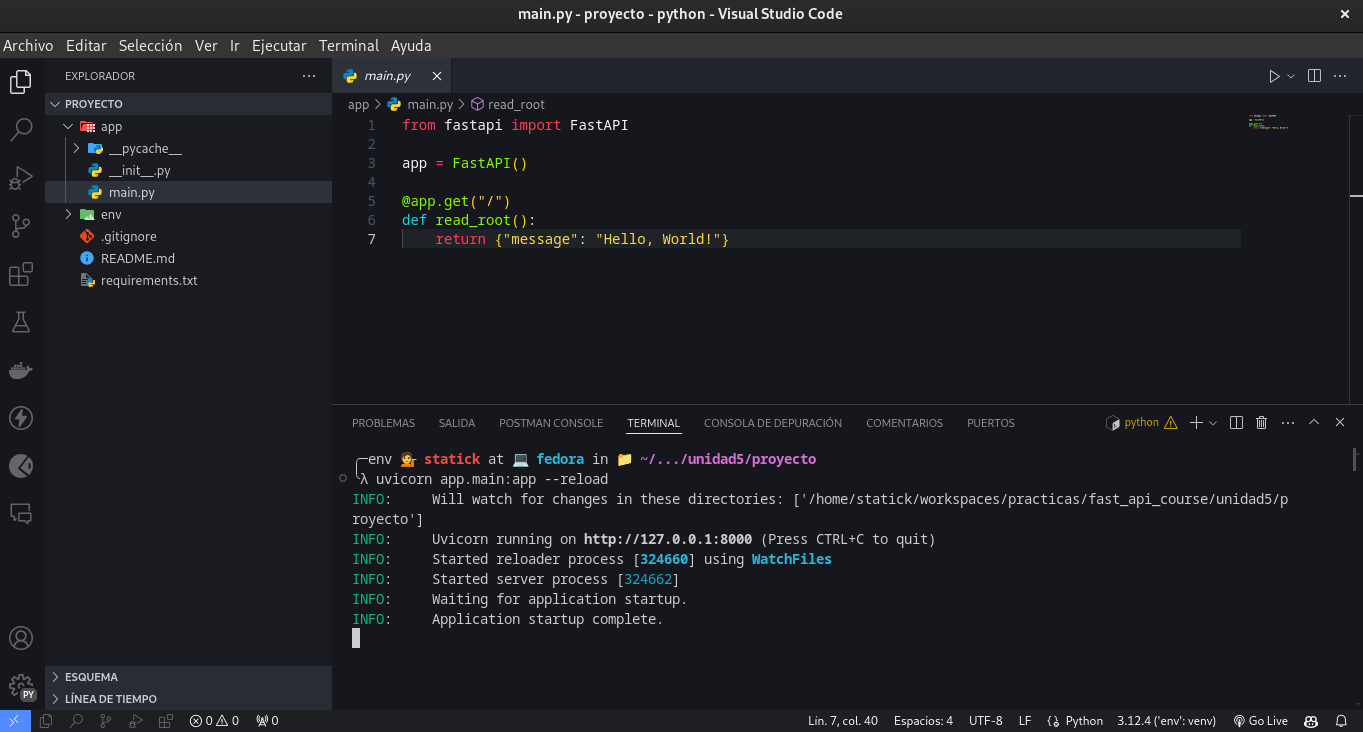
\includegraphics{unidades/unidad5/images/paste-16.png}

\begin{Shaded}
\begin{Highlighting}[]
\ImportTok{from}\NormalTok{ fastapi }\ImportTok{import}\NormalTok{ FastAPI}

\NormalTok{app }\OperatorTok{=}\NormalTok{ FastAPI()}

\AttributeTok{@app.get}\NormalTok{(}\StringTok{"/"}\NormalTok{)}
\KeywordTok{def}\NormalTok{ read\_root():}
    \ControlFlowTok{return}\NormalTok{ \{}\StringTok{"message"}\NormalTok{: }\StringTok{"Hello, World!"}\NormalTok{\}}
\end{Highlighting}
\end{Shaded}

En el ejemplo anterior se importa la clase \textbf{FastAPI} de la
librería \textbf{fastapi} y se crea una instancia de la clase
\textbf{FastAPI} llamada \textbf{app}. A continuación se define una ruta
de la API utilizando el decorador (\textbf{app.get?})\textbf{()} y se
define una operación llamada \textbf{read\_root()} que retorna un
mensaje de bienvenida.

\section{Ejecución de un proyecto
FastAPI}\label{ejecuciuxf3n-de-un-proyecto-fastapi}

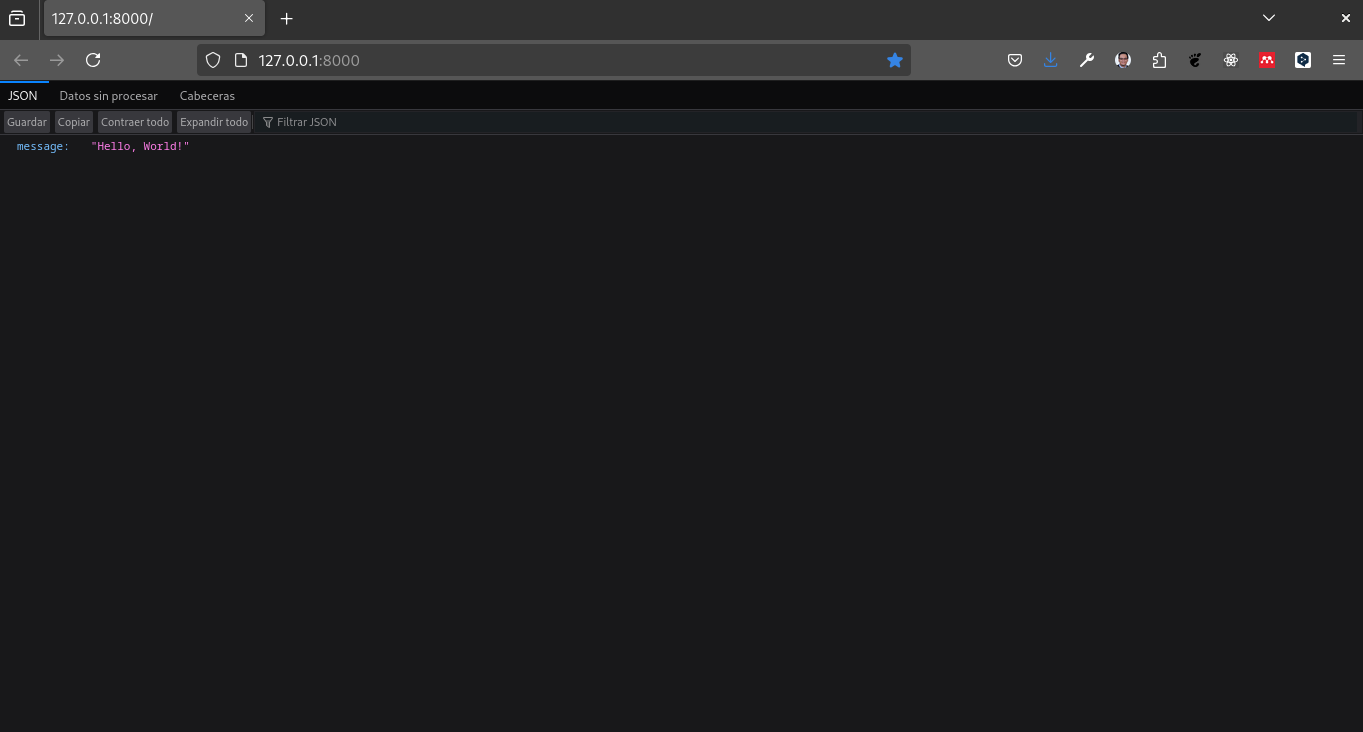
\includegraphics{unidades/unidad5/images/paste-17.png}

Para ejecutar un proyecto FastAPI se utiliza el siguiente comando:

\begin{Shaded}
\begin{Highlighting}[]
\ExtensionTok{uvicorn}\NormalTok{ app.main:app }\AttributeTok{{-}{-}reload}
\end{Highlighting}
\end{Shaded}

En el comando anterior se utiliza el comando \textbf{uvicorn} para
ejecutar el servidor web y se especifica el archivo \textbf{main.py} que
contiene la lógica de la API y la instancia de la clase \textbf{FastAPI}
llamada \textbf{app}. El parámetro \textbf{--reload} indica que el
servidor web se reinicia automáticamente cuando se realizan cambios en
el código fuente.

Al ejecutar el comando anterior se inicia el servidor web y se muestra
la URL de la API en la consola. Para acceder a la API se utiliza la URL
que se muestra en la consola.

\section{Documentación de una API
FastAPI}\label{documentaciuxf3n-de-una-api-fastapi}

FastAPI proporciona una interfaz de usuario interactiva que permite
visualizar y probar la API. Para acceder a la interfaz de usuario se
utiliza la URL de la API seguida de \textbf{/docs}. Por ejemplo, si la
URL de la API es \textbf{http://127.0.0.1:8000}, la URL de la interfaz
de usuario es \textbf{http://127.0.0.1:8000/docs}.

En la interfaz de usuario se muestra una lista de las rutas de la API y
las operaciones que se realizan en cada ruta. Para probar una operación
se hace clic en la operación y se ingresan los parámetros de la
operación.

A continuación se muestra un ejemplo de la interfaz de usuario de
FastAPI:

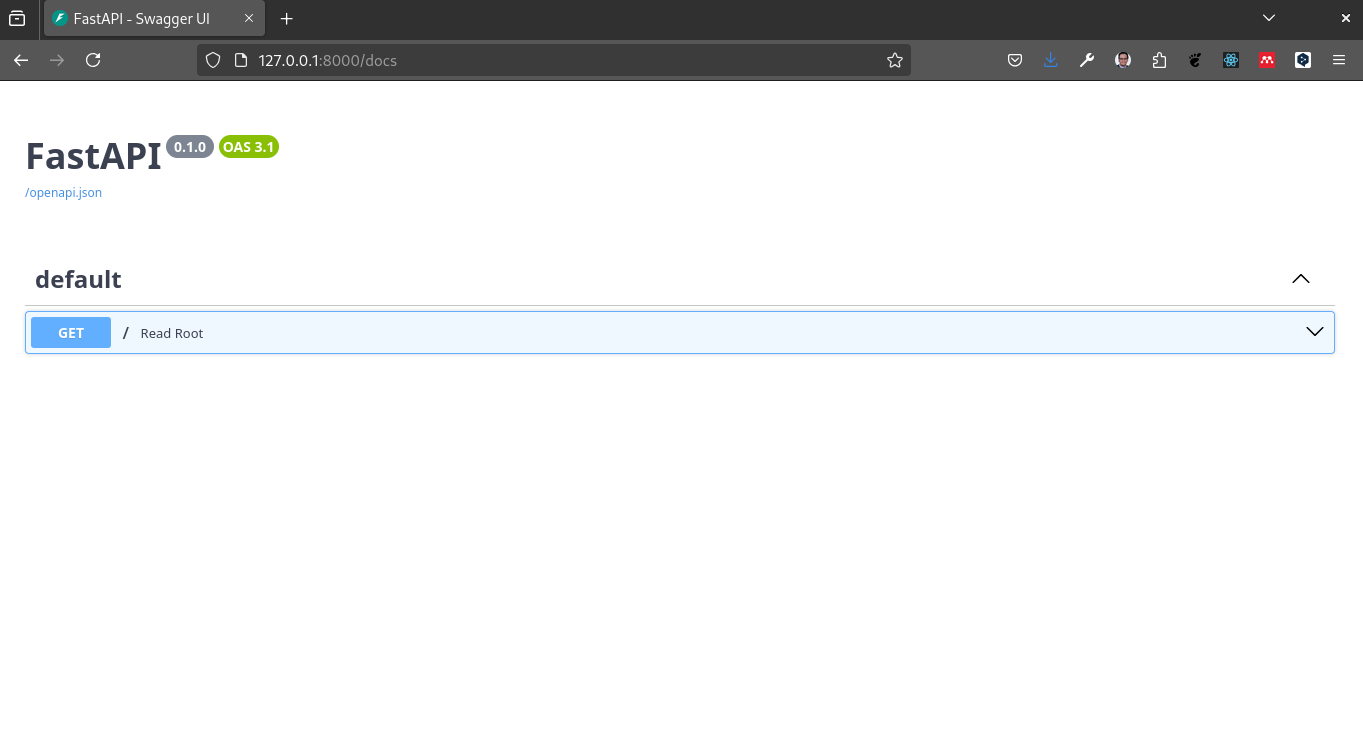
\includegraphics{unidades/unidad5/images/paste-18.png}

En la interfaz de usuario se muestra una lista de las rutas de la API y
las operaciones que se realizan en cada ruta.

FastAPI cuenta con una segunda opción de documentación llamada
\textbf{/redoc} que es una interfaz de usuario alternativa que permite
visualizar y probar la API. Para acceder a la interfaz de usuario
\textbf{redoc} se utiliza la URL de la API seguida de \textbf{/redoc}.
Por ejemplo, si la URL de la API es \textbf{http://127.0.0.1:8000}, la
URL de la interfaz de usuario \textbf{redoc} es
\textbf{http://127.0.0.1:8000/redoc}.

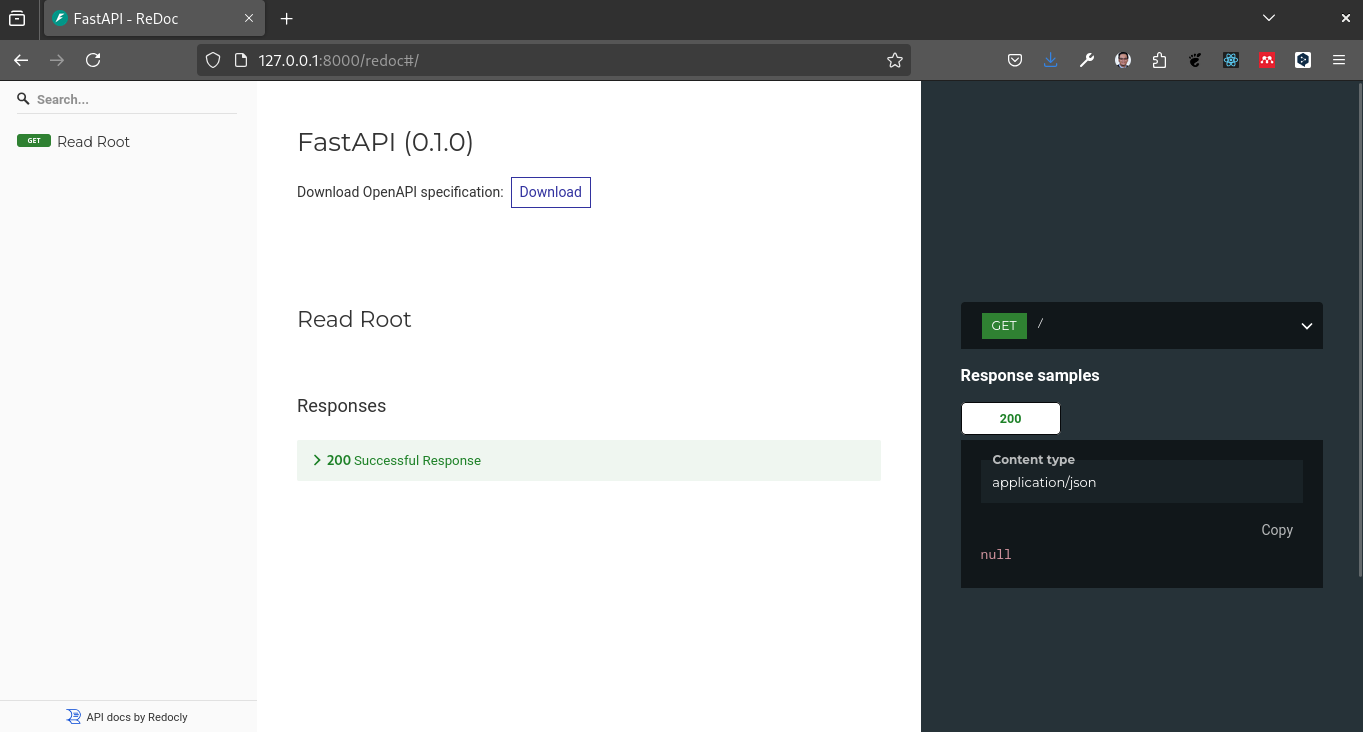
\includegraphics{unidades/unidad5/images/paste-19.png}

En la interfaz de usuario \textbf{redoc} se muestra una lista de las
rutas de la API y las operaciones que se realizan en cada ruta.

En este capítulo se ha mostrado la instalación de FastAPI, la estructura
de un proyecto FastAPI, la ejecución de un proyecto FastAPI y la
documentación de una API FastAPI. En los siguientes capítulos se
mostrará cómo definir rutas y operaciones en FastAPI, cómo validar datos
en FastAPI y cómo trabajar con bases de datos en FastAPI.

\chapter{Pydantic en FastAPI}\label{pydantic-en-fastapi}

\begin{figure}[H]

{\centering \includegraphics[width=2.08333in,height=\textheight]{index_files/mediabag/EEzdj0tm_400x400.jpg}

}

\caption{Pydantic}

\end{figure}%

\section{¿Qué es Pydantic?}\label{quuxe9-es-pydantic}

Pydantic es una librería de Python que permite definir esquemas de datos
y validarlos. Pydantic se utiliza en FastAPI para definir los modelos de
datos que se utilizan en la API y validar los datos que se reciben en
las solicitudes.

En FastAPI se utiliza Pydantic para definir los modelos de datos que se
utilizan en la API. Pydantic es una librería que permite definir
esquemas de datos y validarlos.

La estructura del proyecto de esta unidad es la siguiente:

\begin{Shaded}
\begin{Highlighting}[]
\NormalTok{proyecto/}
\NormalTok{│}
\NormalTok{├── app/}
\NormalTok{│   ├── \_\_init\_\_.py}
\NormalTok{│   ├── main.py}
\NormalTok{│}
\NormalTok{├── .gitignore}
\NormalTok{├── README.md}
\NormalTok{├── requirements.txt}
\end{Highlighting}
\end{Shaded}

A continuación se muestra un ejemplo de cómo definir un modelo de datos
con Pydantic:

Es necesario instalar Pydantic para poder utilizarlo en FastAPI. Para
instalar Pydantic se utiliza el siguiente comando:

\begin{Shaded}
\begin{Highlighting}[]
\ExtensionTok{pip}\NormalTok{ install pydantic}
\end{Highlighting}
\end{Shaded}

Sin olvidar nuestro framework FastAPI:

\begin{Shaded}
\begin{Highlighting}[]
\ExtensionTok{pip}\NormalTok{ install fastapi uvicorn}
\end{Highlighting}
\end{Shaded}

Ahora se puede definir un modelo de datos con Pydantic. A continuación
se muestra un ejemplo de cómo definir un modelo de datos con Pydantic:

\begin{Shaded}
\begin{Highlighting}[]
\ImportTok{from}\NormalTok{ pydantic }\ImportTok{import}\NormalTok{ BaseModel}

\KeywordTok{class}\NormalTok{ Item(BaseModel):}
\NormalTok{    name: }\BuiltInTok{str}
\NormalTok{    price: }\BuiltInTok{float}
\NormalTok{    is\_offer: }\BuiltInTok{bool} \OperatorTok{=} \VariableTok{None}
\end{Highlighting}
\end{Shaded}

En el ejemplo anterior se define un modelo de datos \textbf{Item} que
contiene tres campos: \textbf{name}, \textbf{price} e
\textbf{is\_offer}. El campo \textbf{name} es de tipo \textbf{str}, el
campo \textbf{price} es de tipo \textbf{float} y el campo
\textbf{is\_offer} es de tipo \textbf{bool} con un valor por defecto de
\textbf{None}.

Para utilizar el modelo de datos \textbf{Item} en una operación de la
API se importa la clase \textbf{Item} y se utiliza como tipo de
parámetro en la operación. A continuación se muestra un ejemplo de cómo
utilizar el modelo de datos \textbf{Item} en una operación de la API:

\begin{Shaded}
\begin{Highlighting}[]
\ImportTok{from}\NormalTok{ fastapi }\ImportTok{import}\NormalTok{ FastAPI}
\ImportTok{from}\NormalTok{ pydantic }\ImportTok{import}\NormalTok{ BaseModel}

\NormalTok{app }\OperatorTok{=}\NormalTok{ FastAPI()}

\KeywordTok{class}\NormalTok{ Item(BaseModel):}
\NormalTok{    name: }\BuiltInTok{str}
\NormalTok{    price: }\BuiltInTok{float}
\NormalTok{    is\_offer: }\BuiltInTok{bool} \OperatorTok{=} \VariableTok{None}

\AttributeTok{@app.post}\NormalTok{(}\StringTok{"/items/"}\NormalTok{)}
\ControlFlowTok{async} \KeywordTok{def}\NormalTok{ create\_item(item: Item):}
    \ControlFlowTok{return}\NormalTok{ \{}\StringTok{"name"}\NormalTok{: item.name, }\StringTok{"price"}\NormalTok{: item.price\}}
\end{Highlighting}
\end{Shaded}

En el ejemplo anterior se importa la clase \textbf{Item} y se define una
operación \textbf{create\_item()} que recibe un parámetro \textbf{item}
de tipo \textbf{Item}. En la operación se retorna un diccionario con los
campos \textbf{name} y \textbf{price} del objeto \textbf{item}.

Es necesario probar nuestro código, para ello se ejecuta el servidor web
con el siguiente comando:

\begin{Shaded}
\begin{Highlighting}[]
\ExtensionTok{uvicorn}\NormalTok{ app.main:app }\AttributeTok{{-}{-}reload}
\end{Highlighting}
\end{Shaded}

Para probar la operación \textbf{create\_item()} se puede utilizar una
herramienta como \textbf{Tunder Client} o \textbf{Postman}. A
continuación se muestra un ejemplo de cómo probar la operación
\textbf{create\_item()} con \textbf{Tunder Client}:

Para realizar una solicitud \textbf{POST} a la ruta \textbf{/items/} con
un objeto \textbf{item} se utiliza la siguiente solicitud:

\begin{Shaded}
\begin{Highlighting}[]
\NormalTok{POST /items/}
\NormalTok{Content{-}Type: application/json}

\NormalTok{\{}
\NormalTok{    "name": "item1",}
\NormalTok{    "price": 10.5}
\NormalTok{\}}
\end{Highlighting}
\end{Shaded}

En la solicitud anterior se envía un objeto \textbf{item} con los campos
\textbf{name} y \textbf{price}. La operación \textbf{create\_item()}
recibe el objeto \textbf{item} y retorna un diccionario con los campos
\textbf{name} y \textbf{price} del objeto \textbf{item}.

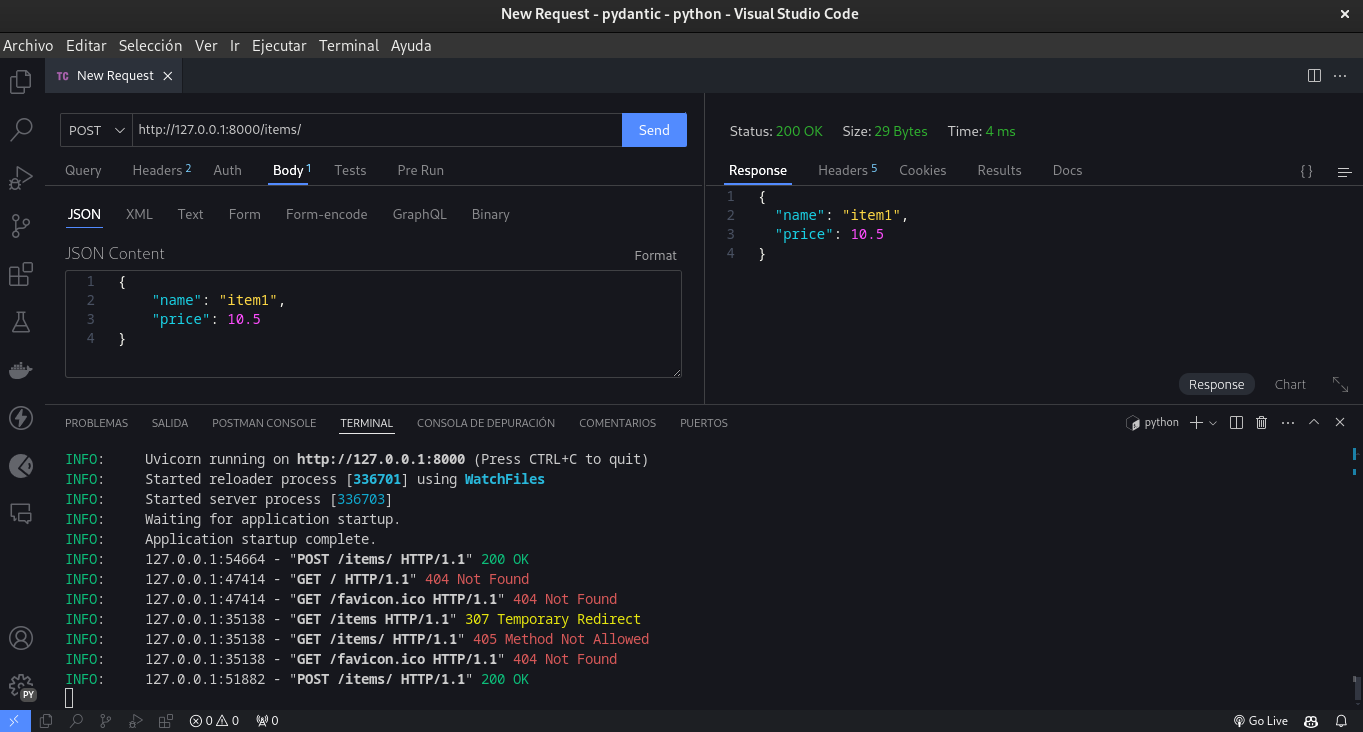
\includegraphics{unidades/unidad5/images/paste-20.png}

En este ejemplo se ha utilizado Pydantic para definir un modelo de datos
\textbf{Item} y validar los datos que se reciben en la solicitud.
Pydantic permite definir esquemas de datos y validarlos, lo que facilita
la creación de APIs con FastAPI.

Para comprobar que todo funciona correctamente, se puede probar la
operación \textbf{create\_item()} con \textbf{Tunder Client} o
\textbf{Postman} y verificar que se retorna un diccionario con los
campos \textbf{name} y \textbf{price} del objeto \textbf{item}.

\chapter{Otro Ejemplo}\label{otro-ejemplo}

En este nuevo ejemplo se va a definir un modelo de datos \textbf{User}
con Pydantic y se va a utilizar un CRUD para la generación de la API. A
continuación se muestra el código del ejemplo:

La estructura del proyecto de esta unidad es la siguiente:

\begin{Shaded}
\begin{Highlighting}[]
\NormalTok{proyecto/}
\NormalTok{│}
\NormalTok{├── app/}
\NormalTok{│   ├── \_\_init\_\_.py}
\NormalTok{│   ├── main.py}
\NormalTok{│}
\NormalTok{├── .gitignore}
\NormalTok{├── README.md}
\NormalTok{├── requirements.txt}
\end{Highlighting}
\end{Shaded}

El código de la API (main.py) es el siguiente:

\begin{Shaded}
\begin{Highlighting}[]
\ImportTok{from}\NormalTok{ fastapi }\ImportTok{import}\NormalTok{ FastAPI}
\ImportTok{from}\NormalTok{ pydantic }\ImportTok{import}\NormalTok{ BaseModel}

\NormalTok{app }\OperatorTok{=}\NormalTok{ FastAPI()}

\KeywordTok{class}\NormalTok{ User(BaseModel):}
    \BuiltInTok{id}\NormalTok{: }\BuiltInTok{int}
\NormalTok{    name: }\BuiltInTok{str}
\NormalTok{    email: }\BuiltInTok{str}

\NormalTok{users }\OperatorTok{=}\NormalTok{ []}

\AttributeTok{@app.post}\NormalTok{(}\StringTok{"/users/"}\NormalTok{)}
\ControlFlowTok{async} \KeywordTok{def}\NormalTok{ create\_user(user: User):}
\NormalTok{    users.append(user)}
    \ControlFlowTok{return}\NormalTok{ user}

\AttributeTok{@app.get}\NormalTok{(}\StringTok{"/users/"}\NormalTok{)}
\ControlFlowTok{async} \KeywordTok{def}\NormalTok{ read\_users():}
    \ControlFlowTok{return}\NormalTok{ users}

\AttributeTok{@app.get}\NormalTok{(}\StringTok{"/users/}\SpecialCharTok{\{user\_id\}}\StringTok{"}\NormalTok{)}
\ControlFlowTok{async} \KeywordTok{def}\NormalTok{ read\_user(user\_id: }\BuiltInTok{int}\NormalTok{):}
    \ControlFlowTok{for}\NormalTok{ user }\KeywordTok{in}\NormalTok{ users:}
        \ControlFlowTok{if}\NormalTok{ user.}\BuiltInTok{id} \OperatorTok{==}\NormalTok{ user\_id:}
            \ControlFlowTok{return}\NormalTok{ user}
    \ControlFlowTok{return}\NormalTok{ \{}\StringTok{"message"}\NormalTok{: }\StringTok{"User not found"}\NormalTok{\}}

\AttributeTok{@app.put}\NormalTok{(}\StringTok{"/users/}\SpecialCharTok{\{user\_id\}}\StringTok{"}\NormalTok{)}
\ControlFlowTok{async} \KeywordTok{def}\NormalTok{ update\_user(user\_id: }\BuiltInTok{int}\NormalTok{, user: User):}
    \ControlFlowTok{for}\NormalTok{ i, u }\KeywordTok{in} \BuiltInTok{enumerate}\NormalTok{(users):}
        \ControlFlowTok{if}\NormalTok{ u.}\BuiltInTok{id} \OperatorTok{==}\NormalTok{ user\_id:}
\NormalTok{            users[i] }\OperatorTok{=}\NormalTok{ user}
            \ControlFlowTok{return}\NormalTok{ user}
    \ControlFlowTok{return}\NormalTok{ \{}\StringTok{"message"}\NormalTok{: }\StringTok{"User not found"}\NormalTok{\}}

\AttributeTok{@app.delete}\NormalTok{(}\StringTok{"/users/}\SpecialCharTok{\{user\_id\}}\StringTok{"}\NormalTok{)}
\ControlFlowTok{async} \KeywordTok{def}\NormalTok{ delete\_user(user\_id: }\BuiltInTok{int}\NormalTok{):}
    \ControlFlowTok{for}\NormalTok{ i, user }\KeywordTok{in} \BuiltInTok{enumerate}\NormalTok{(users):}
        \ControlFlowTok{if}\NormalTok{ user.}\BuiltInTok{id} \OperatorTok{==}\NormalTok{ user\_id:}
            \KeywordTok{del}\NormalTok{ users[i]}
            \ControlFlowTok{return}\NormalTok{ \{}\StringTok{"message"}\NormalTok{: }\StringTok{"User deleted"}\NormalTok{\}}
    \ControlFlowTok{return}\NormalTok{ \{}\StringTok{"message"}\NormalTok{: }\StringTok{"User not found"}\NormalTok{\}}

\ControlFlowTok{if} \VariableTok{\_\_name\_\_} \OperatorTok{==} \StringTok{"\_\_main\_\_"}\NormalTok{:}
    \ImportTok{import}\NormalTok{ uvicorn}
\NormalTok{    uvicorn.run(app, host}\OperatorTok{=}\StringTok{"localhost"}\NormalTok{, port}\OperatorTok{=}\DecValTok{8000}\NormalTok{)}
\end{Highlighting}
\end{Shaded}

En el ejemplo anterior se define un modelo de datos \textbf{User} con
tres campos: \textbf{id}, \textbf{name} y \textbf{email}. Se define una
lista \textbf{users} para almacenar los usuarios y se definen las
operaciones \textbf{create\_user()}, \textbf{read\_users()},
\textbf{read\_user()}, \textbf{update\_user()} y \textbf{delete\_user()}
para realizar las operaciones CRUD sobre los usuarios.

Para probar el ejemplo se ejecuta el servidor web con el siguiente
comando:

\begin{Shaded}
\begin{Highlighting}[]
\ExtensionTok{uvicorn}\NormalTok{ app.main:app }\AttributeTok{{-}{-}reload}
\end{Highlighting}
\end{Shaded}

Para probar las operaciones CRUD sobre los usuarios se puede utilizar
una herramienta como \textbf{Tunder Client} o \textbf{Postman}. A
continuación se muestra un ejemplo de cómo probar las operaciones CRUD
sobre los usuarios con \textbf{Tunder Client}:

Para crear un usuario se realiza una solicitud \textbf{POST} a la ruta
\textbf{/users/} con un objeto \textbf{user}:

\begin{Shaded}
\begin{Highlighting}[]
\NormalTok{POST /users/}
\NormalTok{Content{-}Type: application/json}

\NormalTok{\{}
\NormalTok{    "id": 1,}
\NormalTok{    "name": "user1",}
\NormalTok{    "email": "dmsaavedra@espe.edu.ec"}
\NormalTok{\}}
\end{Highlighting}
\end{Shaded}

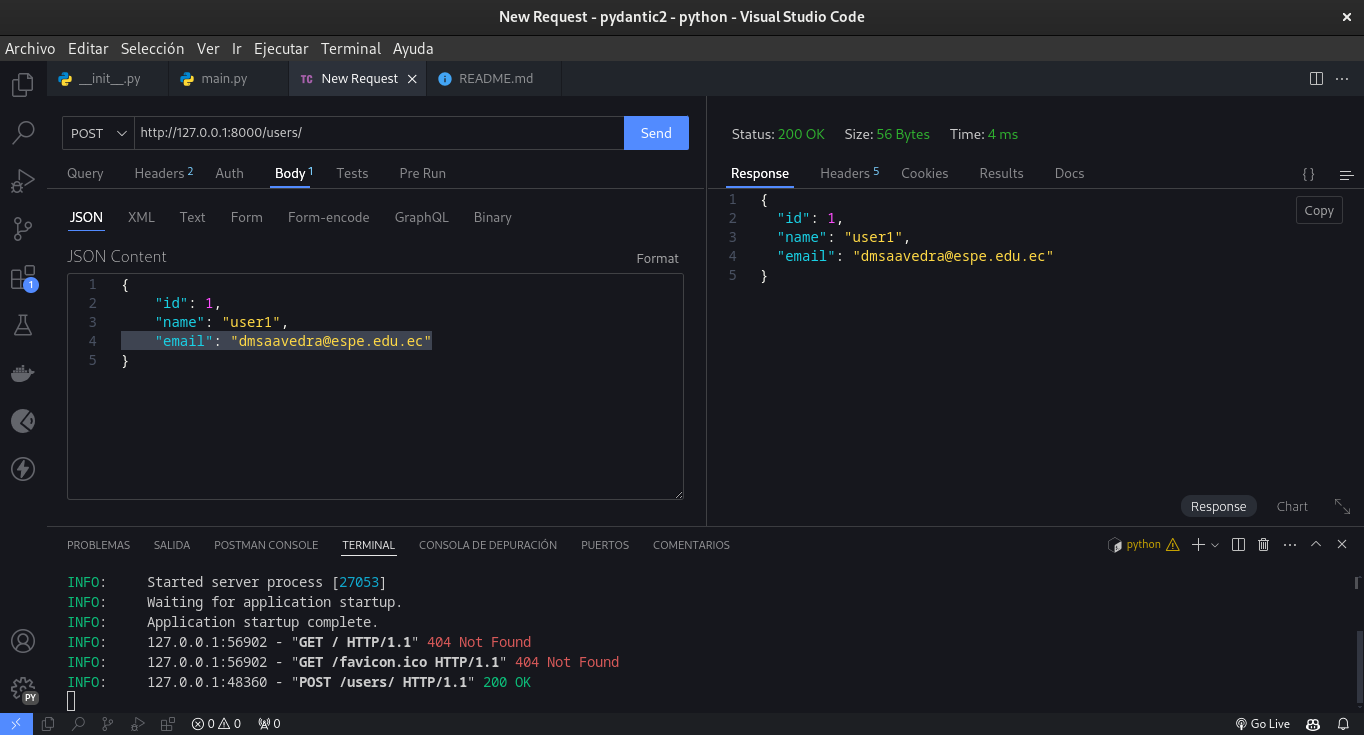
\includegraphics{unidades/unidad5/images/paste-21.png}

Para obtener todos los usuarios se realiza una solicitud \textbf{GET} a
la ruta \textbf{/users/}:

\begin{Shaded}
\begin{Highlighting}[]
\NormalTok{GET /users/}
\end{Highlighting}
\end{Shaded}

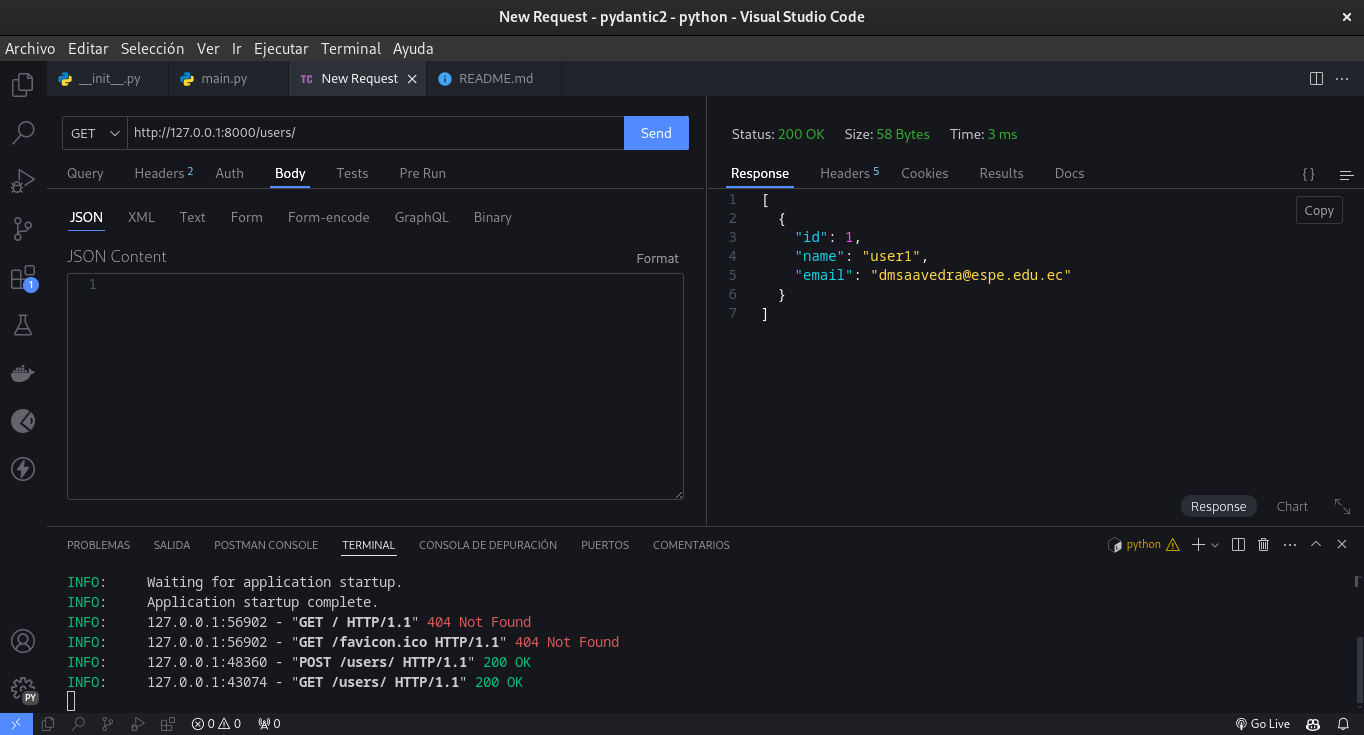
\includegraphics{unidades/unidad5/images/paste-22.png}

Para obtener un usuario se realiza una solicitud \textbf{GET} a la ruta
\textbf{/users/\{user\_id\}} con el \textbf{id} del usuario:

\begin{Shaded}
\begin{Highlighting}[]
\NormalTok{GET /users/1}
\end{Highlighting}
\end{Shaded}

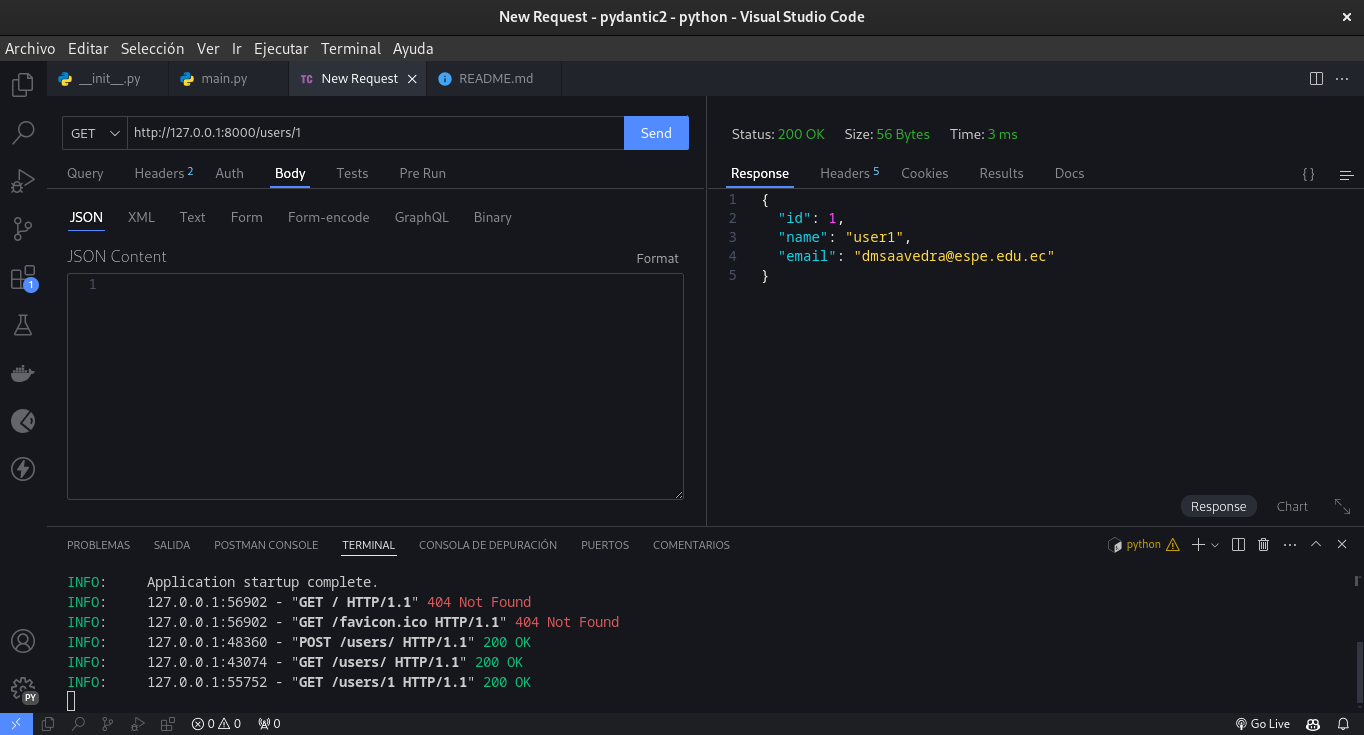
\includegraphics{unidades/unidad5/images/paste-23.png}

Para actualizar un usuario se realiza una solicitud \textbf{PUT} a la
ruta \textbf{/users/\{user\_id\}} con el \textbf{id} del usuario y un
objeto \textbf{user}:

\begin{Shaded}
\begin{Highlighting}[]
\NormalTok{PUT /users/1}
\NormalTok{Content{-}Type: application/json}

\NormalTok{\{}
\NormalTok{    "id": 1,}
\NormalTok{    "name": "user2",}
\NormalTok{    "email": "dmsaavedra@espe.edu.ec"}
\NormalTok{\}}
\end{Highlighting}
\end{Shaded}

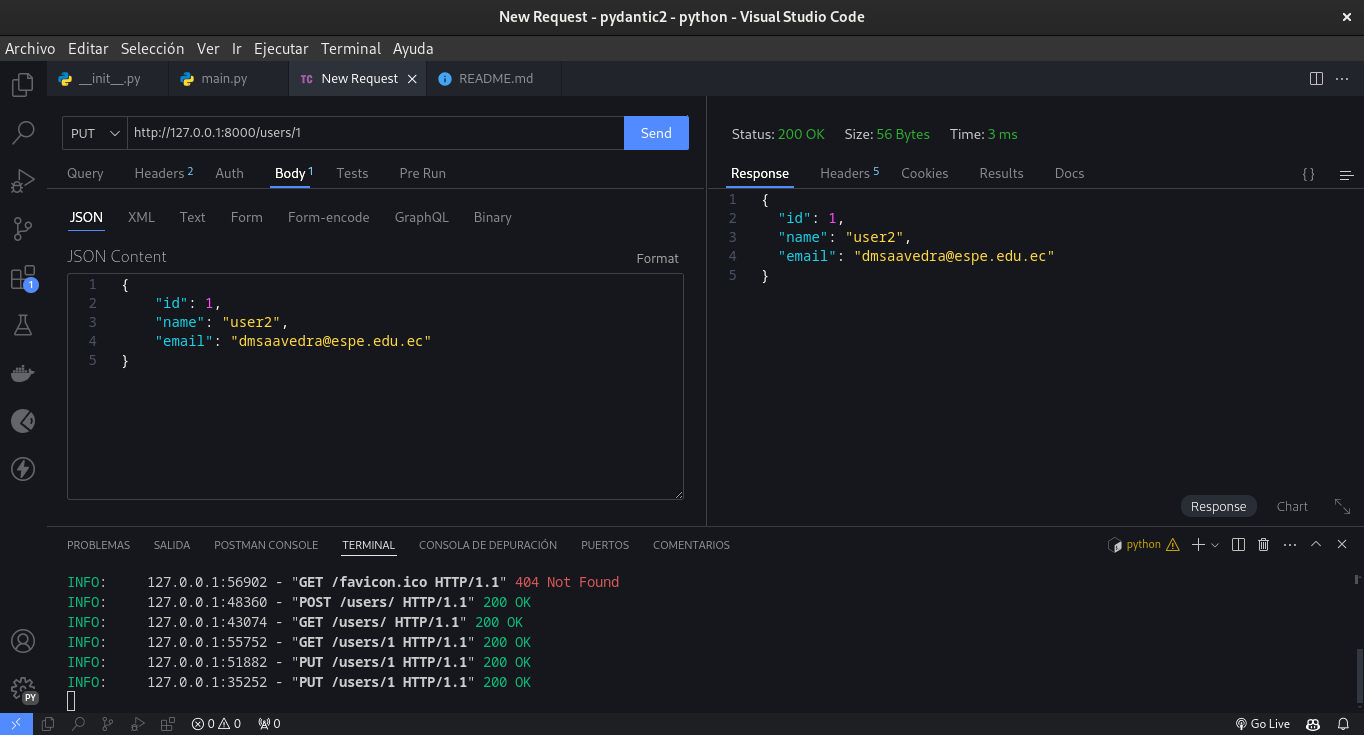
\includegraphics{unidades/unidad5/images/paste-24.png}

Para eliminar un usuario se realiza una solicitud \textbf{DELETE} a la
ruta \textbf{/users/\{user\_id\}} con el \textbf{id} del usuario:

\begin{Shaded}
\begin{Highlighting}[]
\NormalTok{DELETE /users/1}
\end{Highlighting}
\end{Shaded}

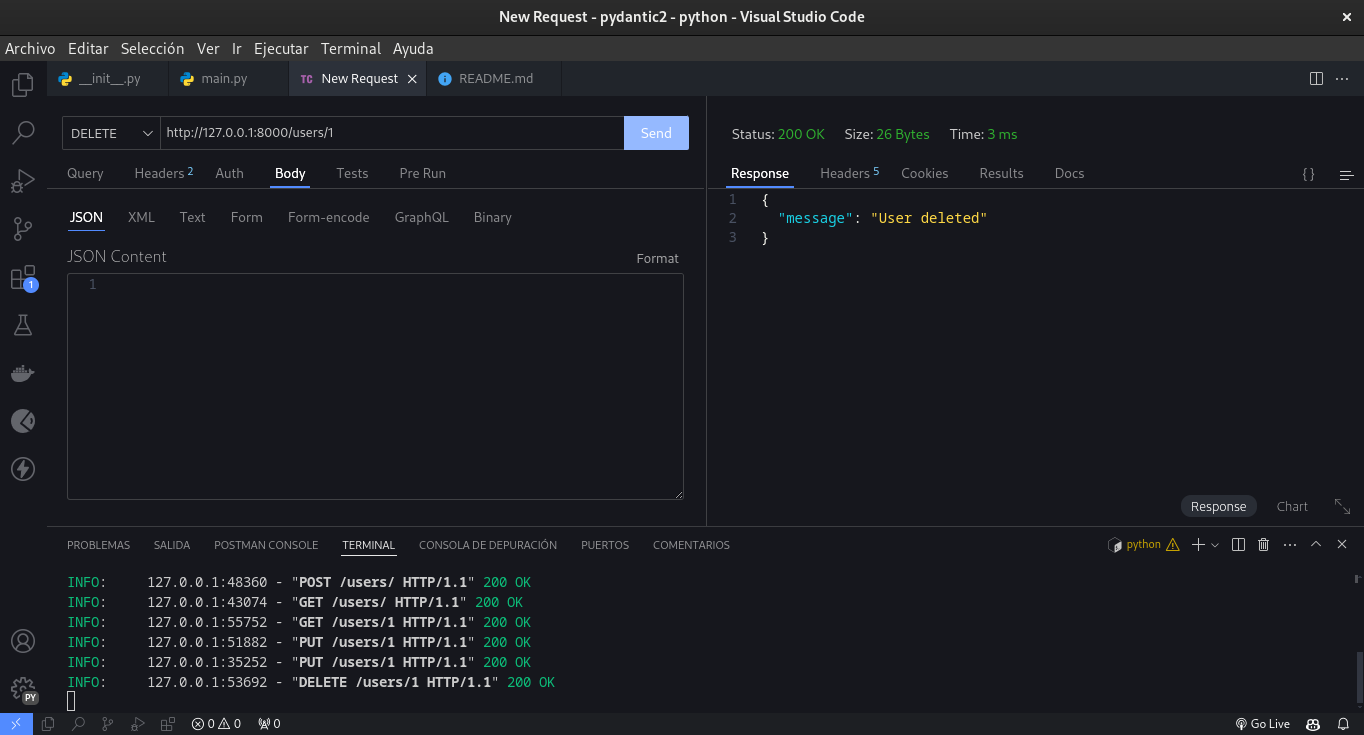
\includegraphics{unidades/unidad5/images/paste-25.png}

En este ejemplo se ha utilizado Pydantic para definir un modelo de datos
\textbf{User} y validar los datos que se reciben en las solicitudes.
Pydantic permite definir esquemas de datos y validarlos, lo que facilita
la creación de APIs con FastAPI.

En este capítulo se ha mostrado cómo utilizar Pydantic en FastAPI para
definir modelos de datos y validar los datos que se reciben en las
solicitudes. Pydantic es una librería de Python que permite definir
esquemas de datos y validarlos, lo que facilita la creación de APIs con
FastAPI.

\chapter{Modelos en FastAPI}\label{modelos-en-fastapi}

\part{Unidad 6: Desarrollo Avanzado en FastAPI}

\chapter{Rutas y Validaciones en
FastAPI}\label{rutas-y-validaciones-en-fastapi}

\chapter{APIs RESTful con FastAPI}\label{apis-restful-con-fastapi}

\chapter{Pruebas Unitarias en
FastAPI}\label{pruebas-unitarias-en-fastapi}

\chapter{Optimización y
Rendimiento}\label{optimizaciuxf3n-y-rendimiento}

\chapter{Creación de una API de gestión de tareas utilizando
FastAPI}\label{creaciuxf3n-de-una-api-de-gestiuxf3n-de-tareas-utilizando-fastapi}

\part{Unidad 7: Consumo API con FastAPI}

\chapter{Configuración y Uso de FastAPI para consumir
APIs}\label{configuraciuxf3n-y-uso-de-fastapi-para-consumir-apis}

\chapter{Integración de APIs de terceros con
FastAPI}\label{integraciuxf3n-de-apis-de-terceros-con-fastapi}

\part{Unidad 8: Desarrollo Avanzado}

\chapter{Manejo de Estado en FastAPI, Context
API}\label{manejo-de-estado-en-fastapi-context-api}

\chapter{Navegación en FastAPI con
FastRouter}\label{navegaciuxf3n-en-fastapi-con-fastrouter}

\chapter{Aplicación en FastAPI que consume APIs de
terceros}\label{aplicaciuxf3n-en-fastapi-que-consume-apis-de-terceros}

\part{Unidad 9: Prácticas Avanadas de Programación}

\chapter{Patrones de Diseño en
FastAPI}\label{patrones-de-diseuxf1o-en-fastapi}

\chapter{Arquitectura de Software y Diseño
Modular}\label{arquitectura-de-software-y-diseuxf1o-modular}

\part{Proyecto Final}

\chapter{}\label{section}

\chapter{}\label{section-1}

\chapter{}\label{section-2}

\part{Laboratorios}

\chapter{Desarrollo del Backend para un E-Commerce con Django Rest
Framework}\label{desarrollo-del-backend-para-un-e-commerce-con-django-rest-framework}

\section{1. Configuración Inicial del
Proyecto}\label{configuraciuxf3n-inicial-del-proyecto}

\subsection{1.1. Crear un Proyecto
Django}\label{crear-un-proyecto-django}

Abre tu terminal y ejecuta los siguientes comandos para crear un nuevo
proyecto Django:

\begin{Shaded}
\begin{Highlighting}[]
\ExtensionTok{python} \AttributeTok{{-}m}\NormalTok{ venv env}
\BuiltInTok{source}\NormalTok{ env/bin/activate}
\ExtensionTok{pip}\NormalTok{ install django==4.2}
\ExtensionTok{django{-}admin}\NormalTok{ startproject ecommerce\_project .}
\BuiltInTok{cd}\NormalTok{ ecommerce\_project}
\end{Highlighting}
\end{Shaded}

\subsection{1.2 Crear una Aplicación
Django}\label{crear-una-aplicaciuxf3n-django}

Dentro del directorio del proyecto, crea una aplicación para manejar el
e-commerce:

\begin{Shaded}
\begin{Highlighting}[]
\ExtensionTok{python}\NormalTok{ manage.py startapp products}
\end{Highlighting}
\end{Shaded}

\subsection{1.3 Instalar Django Rest
Framework}\label{instalar-django-rest-framework}

Instala DRF usando pip:

\begin{Shaded}
\begin{Highlighting}[]
\ExtensionTok{pip}\NormalTok{ install djangorestframework}
\end{Highlighting}
\end{Shaded}

\subsection{1.4 Configurar el Proyecto}\label{configurar-el-proyecto}

Añade `rest\_framework' y tu nueva aplicación `products' a la lista
INSTALLED\_APPS en ecommerce\_project/settings.py:

\begin{Shaded}
\begin{Highlighting}[]
\NormalTok{INSTALLED\_APPS }\OperatorTok{=}\NormalTok{ [}
    \CommentTok{\# ... otras apps}
    \StringTok{\textquotesingle{}rest\_framework\textquotesingle{}}\NormalTok{,}
    \StringTok{\textquotesingle{}products\textquotesingle{}}\NormalTok{,}
\NormalTok{]}
\end{Highlighting}
\end{Shaded}

\section{2. Definir el Modelo de
Datos}\label{definir-el-modelo-de-datos}

\subsection{2.1 Crear Modelos en
products/models.py}\label{crear-modelos-en-productsmodels.py}

Define los modelos para el e-commerce, como Product, Category, y Order:

\begin{Shaded}
\begin{Highlighting}[]
\ImportTok{from}\NormalTok{ django.db }\ImportTok{import}\NormalTok{ models}

\KeywordTok{class}\NormalTok{ Category(models.Model):}
\NormalTok{    name }\OperatorTok{=}\NormalTok{ models.CharField(max\_length}\OperatorTok{=}\DecValTok{100}\NormalTok{)}

    \KeywordTok{def} \FunctionTok{\_\_str\_\_}\NormalTok{(}\VariableTok{self}\NormalTok{):}
        \ControlFlowTok{return} \VariableTok{self}\NormalTok{.name}

\KeywordTok{class}\NormalTok{ Product(models.Model):}
\NormalTok{    name }\OperatorTok{=}\NormalTok{ models.CharField(max\_length}\OperatorTok{=}\DecValTok{100}\NormalTok{)}
\NormalTok{    description }\OperatorTok{=}\NormalTok{ models.TextField()}
\NormalTok{    price }\OperatorTok{=}\NormalTok{ models.DecimalField(max\_digits}\OperatorTok{=}\DecValTok{10}\NormalTok{, decimal\_places}\OperatorTok{=}\DecValTok{2}\NormalTok{)}
\NormalTok{    category }\OperatorTok{=}\NormalTok{ models.ForeignKey(Category, related\_name}\OperatorTok{=}\StringTok{\textquotesingle{}products\textquotesingle{}}\NormalTok{, on\_delete}\OperatorTok{=}\NormalTok{models.CASCADE)}
\NormalTok{    stock }\OperatorTok{=}\NormalTok{ models.PositiveIntegerField()}

    \KeywordTok{def} \FunctionTok{\_\_str\_\_}\NormalTok{(}\VariableTok{self}\NormalTok{):}
        \ControlFlowTok{return} \VariableTok{self}\NormalTok{.name}

\KeywordTok{class}\NormalTok{ Order(models.Model):}
\NormalTok{    product }\OperatorTok{=}\NormalTok{ models.ForeignKey(Product, related\_name}\OperatorTok{=}\StringTok{\textquotesingle{}orders\textquotesingle{}}\NormalTok{, on\_delete}\OperatorTok{=}\NormalTok{models.CASCADE)}
\NormalTok{    quantity }\OperatorTok{=}\NormalTok{ models.PositiveIntegerField()}
\NormalTok{    total\_price }\OperatorTok{=}\NormalTok{ models.DecimalField(max\_digits}\OperatorTok{=}\DecValTok{10}\NormalTok{, decimal\_places}\OperatorTok{=}\DecValTok{2}\NormalTok{)}
\NormalTok{    order\_date }\OperatorTok{=}\NormalTok{ models.DateTimeField(auto\_now\_add}\OperatorTok{=}\VariableTok{True}\NormalTok{)}

    \KeywordTok{def} \FunctionTok{\_\_str\_\_}\NormalTok{(}\VariableTok{self}\NormalTok{):}
        \ControlFlowTok{return} \SpecialStringTok{f"Order }\SpecialCharTok{\{}\VariableTok{self}\SpecialCharTok{.}\BuiltInTok{id}\SpecialCharTok{\}}\SpecialStringTok{ {-} }\SpecialCharTok{\{}\VariableTok{self}\SpecialCharTok{.}\NormalTok{product}\SpecialCharTok{.}\NormalTok{name}\SpecialCharTok{\}}\SpecialStringTok{"}
\end{Highlighting}
\end{Shaded}

\subsection{2.2 Crear y Aplicar
Migraciones}\label{crear-y-aplicar-migraciones}

Genera y aplica las migraciones para los modelos:

\begin{Shaded}
\begin{Highlighting}[]
\ExtensionTok{python}\NormalTok{ manage.py makemigrations}
\ExtensionTok{python}\NormalTok{ manage.py migrate}
\end{Highlighting}
\end{Shaded}

\section{3. Crear Serializers}\label{crear-serializers}

\subsection{3.1 Definir Serializers en
products/serializers.py}\label{definir-serializers-en-productsserializers.py}

Los serializers se encargan de transformar los modelos en formatos JSON
y viceversa:

\begin{Shaded}
\begin{Highlighting}[]
\ImportTok{from}\NormalTok{ rest\_framework }\ImportTok{import}\NormalTok{ serializers}
\ImportTok{from}\NormalTok{ .models }\ImportTok{import}\NormalTok{ Category, Product, Order}

\KeywordTok{class}\NormalTok{ CategorySerializer(serializers.ModelSerializer):}
    \KeywordTok{class}\NormalTok{ Meta:}
\NormalTok{        model }\OperatorTok{=}\NormalTok{ Category}
\NormalTok{        fields }\OperatorTok{=} \StringTok{\textquotesingle{}\_\_all\_\_\textquotesingle{}}

\KeywordTok{class}\NormalTok{ ProductSerializer(serializers.ModelSerializer):}
\NormalTok{    category }\OperatorTok{=}\NormalTok{ CategorySerializer()}

    \KeywordTok{class}\NormalTok{ Meta:}
\NormalTok{        model }\OperatorTok{=}\NormalTok{ Product}
\NormalTok{        fields }\OperatorTok{=} \StringTok{\textquotesingle{}\_\_all\_\_\textquotesingle{}}

\KeywordTok{class}\NormalTok{ OrderSerializer(serializers.ModelSerializer):}
\NormalTok{    product }\OperatorTok{=}\NormalTok{ ProductSerializer()}

    \KeywordTok{class}\NormalTok{ Meta:}
\NormalTok{        model }\OperatorTok{=}\NormalTok{ Order}
\NormalTok{        fields }\OperatorTok{=} \StringTok{\textquotesingle{}\_\_all\_\_\textquotesingle{}}
\end{Highlighting}
\end{Shaded}

\section{4. Crear Vistas y Rutas}\label{crear-vistas-y-rutas}

\subsection{4.1 Definir Vistas en
products/views.py}\label{definir-vistas-en-productsviews.py}

Utiliza las vistas basadas en clases de DRF para crear y manejar las
operaciones CRUD:

\begin{Shaded}
\begin{Highlighting}[]
\ImportTok{from}\NormalTok{ rest\_framework }\ImportTok{import}\NormalTok{ generics}
\ImportTok{from}\NormalTok{ .models }\ImportTok{import}\NormalTok{ Category, Product, Order}
\ImportTok{from}\NormalTok{ .serializers }\ImportTok{import}\NormalTok{ CategorySerializer, ProductSerializer, OrderSerializer}

\KeywordTok{class}\NormalTok{ CategoryListCreate(generics.ListCreateAPIView):}
\NormalTok{    queryset }\OperatorTok{=}\NormalTok{ Category.objects.}\BuiltInTok{all}\NormalTok{()}
\NormalTok{    serializer\_class }\OperatorTok{=}\NormalTok{ CategorySerializer}

\KeywordTok{class}\NormalTok{ CategoryDetail(generics.RetrieveUpdateDestroyAPIView):}
\NormalTok{    queryset }\OperatorTok{=}\NormalTok{ Category.objects.}\BuiltInTok{all}\NormalTok{()}
\NormalTok{    serializer\_class }\OperatorTok{=}\NormalTok{ CategorySerializer}

\KeywordTok{class}\NormalTok{ ProductListCreate(generics.ListCreateAPIView):}
\NormalTok{    queryset }\OperatorTok{=}\NormalTok{ Product.objects.}\BuiltInTok{all}\NormalTok{()}
\NormalTok{    serializer\_class }\OperatorTok{=}\NormalTok{ ProductSerializer}

\KeywordTok{class}\NormalTok{ ProductDetail(generics.RetrieveUpdateDestroyAPIView):}
\NormalTok{    queryset }\OperatorTok{=}\NormalTok{ Product.objects.}\BuiltInTok{all}\NormalTok{()}
\NormalTok{    serializer\_class }\OperatorTok{=}\NormalTok{ ProductSerializer}

\KeywordTok{class}\NormalTok{ OrderListCreate(generics.ListCreateAPIView):}
\NormalTok{    queryset }\OperatorTok{=}\NormalTok{ Order.objects.}\BuiltInTok{all}\NormalTok{()}
\NormalTok{    serializer\_class }\OperatorTok{=}\NormalTok{ OrderSerializer}

\KeywordTok{class}\NormalTok{ OrderDetail(generics.RetrieveUpdateDestroyAPIView):}
\NormalTok{    queryset }\OperatorTok{=}\NormalTok{ Order.objects.}\BuiltInTok{all}\NormalTok{()}
\NormalTok{    serializer\_class }\OperatorTok{=}\NormalTok{ OrderSerializer}
\end{Highlighting}
\end{Shaded}

\section{4.2 Configurar Rutas en
products/urls.py}\label{configurar-rutas-en-productsurls.py}

Define las rutas para acceder a las vistas:

\begin{Shaded}
\begin{Highlighting}[]
\ImportTok{from}\NormalTok{ django.urls }\ImportTok{import}\NormalTok{ path}
\ImportTok{from}\NormalTok{ . }\ImportTok{import}\NormalTok{ views}

\NormalTok{urlpatterns }\OperatorTok{=}\NormalTok{ [}
\NormalTok{    path(}\StringTok{\textquotesingle{}categories/\textquotesingle{}}\NormalTok{, views.CategoryListCreate.as\_view(), name}\OperatorTok{=}\StringTok{\textquotesingle{}category{-}list{-}create\textquotesingle{}}\NormalTok{),}
\NormalTok{    path(}\StringTok{\textquotesingle{}categories/\textless{}int:pk\textgreater{}/\textquotesingle{}}\NormalTok{, views.CategoryDetail.as\_view(), name}\OperatorTok{=}\StringTok{\textquotesingle{}category{-}detail\textquotesingle{}}\NormalTok{),}
\NormalTok{    path(}\StringTok{\textquotesingle{}products/\textquotesingle{}}\NormalTok{, views.ProductListCreate.as\_view(), name}\OperatorTok{=}\StringTok{\textquotesingle{}product{-}list{-}create\textquotesingle{}}\NormalTok{),}
\NormalTok{    path(}\StringTok{\textquotesingle{}products/\textless{}int:pk\textgreater{}/\textquotesingle{}}\NormalTok{, views.ProductDetail.as\_view(), name}\OperatorTok{=}\StringTok{\textquotesingle{}product{-}detail\textquotesingle{}}\NormalTok{),}
\NormalTok{    path(}\StringTok{\textquotesingle{}orders/\textquotesingle{}}\NormalTok{, views.OrderListCreate.as\_view(), name}\OperatorTok{=}\StringTok{\textquotesingle{}order{-}list{-}create\textquotesingle{}}\NormalTok{),}
\NormalTok{    path(}\StringTok{\textquotesingle{}orders/\textless{}int:pk\textgreater{}/\textquotesingle{}}\NormalTok{, views.OrderDetail.as\_view(), name}\OperatorTok{=}\StringTok{\textquotesingle{}order{-}detail\textquotesingle{}}\NormalTok{),}
\NormalTok{]}
\end{Highlighting}
\end{Shaded}

\section{4.3 Incluir las URLs en
ecommerce\_project/urls.py}\label{incluir-las-urls-en-ecommerce_projecturls.py}

Añade las URLs de la aplicación al archivo principal de URLs del
proyecto:

\begin{Shaded}
\begin{Highlighting}[]
\ImportTok{from}\NormalTok{ django.contrib }\ImportTok{import}\NormalTok{ admin}
\ImportTok{from}\NormalTok{ django.urls }\ImportTok{import}\NormalTok{ path, include}

\NormalTok{urlpatterns }\OperatorTok{=}\NormalTok{ [}
\NormalTok{    path(}\StringTok{\textquotesingle{}admin/\textquotesingle{}}\NormalTok{, admin.site.urls),}
\NormalTok{    path(}\StringTok{\textquotesingle{}api/\textquotesingle{}}\NormalTok{, include(}\StringTok{\textquotesingle{}products.urls\textquotesingle{}}\NormalTok{)),}
\NormalTok{]}
\end{Highlighting}
\end{Shaded}

\section{5. Probar la API}\label{probar-la-api}

\subsection{5.1 Ejecutar el Servidor de
Desarrollo}\label{ejecutar-el-servidor-de-desarrollo}

Inicia el servidor de desarrollo de Django:

\begin{Shaded}
\begin{Highlighting}[]
\ExtensionTok{python}\NormalTok{ manage.py runserver}
\end{Highlighting}
\end{Shaded}

\section{5.2 Probar los Endpoints}\label{probar-los-endpoints}

Utiliza herramientas como Postman o cURL para probar los endpoints:

\begin{itemize}
\tightlist
\item
  Listar categorías: GET /api/categories/
\item
  Crear categoría: POST /api/categories/
\item
  Obtener categoría específica: GET /api/categories/\{id\}/
\item
  Actualizar categoría: PUT /api/categories/\{id\}/
\item
  Eliminar categoría: DELETE /api/categories/\{id\}/
\end{itemize}

Y lo mismo para productos y pedidos.

\begin{itemize}
\tightlist
\item
  Listar productos: GET /api/products/
\item
  Crear producto: POST /api/products/
\item
  Obtener producto específico: GET /api/products/\{id\}/
\item
  Actualizar producto: PUT /api/products/\{id\}/
\item
  Eliminar producto: DELETE /api/products/\{id\}/
\end{itemize}

\chapter{Extra}\label{extra}

Agreguemos Swagger a nuestro proyecto para tener una documentación de
nuestra API.

\section{1. Instalar Django Rest
Swagger}\label{instalar-django-rest-swagger}

Instala Django Rest Swagger usando pip:

\begin{Shaded}
\begin{Highlighting}[]
\ExtensionTok{pip}\NormalTok{ install drf{-}yasg}
\end{Highlighting}
\end{Shaded}

\section{2. Configurar Django Rest
Swagger}\label{configurar-django-rest-swagger}

Añade `rest\_framework\_swagger' a la lista INSTALLED\_APPS en
ecommerce\_project/settings.py:

\begin{Shaded}
\begin{Highlighting}[]
\ImportTok{from}\NormalTok{ django.contrib }\ImportTok{import}\NormalTok{ admin}
\ImportTok{from}\NormalTok{ django.urls }\ImportTok{import}\NormalTok{ path, include}
\ImportTok{from}\NormalTok{ rest\_framework }\ImportTok{import}\NormalTok{ permissions}
\ImportTok{from}\NormalTok{ drf\_yasg.views }\ImportTok{import}\NormalTok{ get\_schema\_view}
\ImportTok{from}\NormalTok{ drf\_yasg }\ImportTok{import}\NormalTok{ openapi}

\NormalTok{schema\_view }\OperatorTok{=}\NormalTok{ get\_schema\_view(}
\NormalTok{    openapi.Info(}
\NormalTok{        title}\OperatorTok{=}\StringTok{"E{-}commerce API"}\NormalTok{,}
\NormalTok{        default\_version}\OperatorTok{=}\StringTok{\textquotesingle{}v1\textquotesingle{}}\NormalTok{,}
\NormalTok{        description}\OperatorTok{=}\StringTok{"API documentation for the E{-}commerce project"}\NormalTok{,}
\NormalTok{        terms\_of\_service}\OperatorTok{=}\StringTok{"https://www.google.com/policies/terms/"}\NormalTok{,}
\NormalTok{        contact}\OperatorTok{=}\NormalTok{openapi.Contact(email}\OperatorTok{=}\StringTok{"contact@ecommerce.local"}\NormalTok{),}
\NormalTok{        license}\OperatorTok{=}\NormalTok{openapi.License(name}\OperatorTok{=}\StringTok{"BSD License"}\NormalTok{),}
\NormalTok{    ),}
\NormalTok{    public}\OperatorTok{=}\VariableTok{True}\NormalTok{,}
\NormalTok{    permission\_classes}\OperatorTok{=}\NormalTok{(permissions.AllowAny,),}
\NormalTok{)}

\NormalTok{urlpatterns }\OperatorTok{=}\NormalTok{ [}
\NormalTok{    path(}\StringTok{\textquotesingle{}admin/\textquotesingle{}}\NormalTok{, admin.site.urls),}
\NormalTok{    path(}\StringTok{\textquotesingle{}api/\textquotesingle{}}\NormalTok{, include(}\StringTok{\textquotesingle{}products.urls\textquotesingle{}}\NormalTok{)),}
\NormalTok{    path(}\StringTok{\textquotesingle{}docs/\textquotesingle{}}\NormalTok{, schema\_view.with\_ui(}\StringTok{\textquotesingle{}swagger\textquotesingle{}}\NormalTok{, cache\_timeout}\OperatorTok{=}\DecValTok{0}\NormalTok{), name}\OperatorTok{=}\StringTok{\textquotesingle{}schema{-}swagger{-}ui\textquotesingle{}}\NormalTok{),}
\NormalTok{    path(}\StringTok{\textquotesingle{}redoc/\textquotesingle{}}\NormalTok{, schema\_view.with\_ui(}\StringTok{\textquotesingle{}redoc\textquotesingle{}}\NormalTok{, cache\_timeout}\OperatorTok{=}\DecValTok{0}\NormalTok{), name}\OperatorTok{=}\StringTok{\textquotesingle{}schema{-}redoc\textquotesingle{}}\NormalTok{),}
\NormalTok{]}
\end{Highlighting}
\end{Shaded}

\section{3. Configurar las URLs}\label{configurar-las-urls}

Añade las URLs de Swagger al archivo principal de URLs del proyecto:

\begin{Shaded}
\begin{Highlighting}[]
\NormalTok{´´´}
\ImportTok{from}\NormalTok{ rest\_framework\_swagger.views }\ImportTok{import}\NormalTok{ get\_swagger\_view}

\NormalTok{schema\_view }\OperatorTok{=}\NormalTok{ get\_swagger\_view(title}\OperatorTok{=}\StringTok{\textquotesingle{}E{-}Commerce API\textquotesingle{}}\NormalTok{)}

\NormalTok{urlpatterns }\OperatorTok{=}\NormalTok{ [}
\NormalTok{    ´´´}
\NormalTok{    path(}\StringTok{\textquotesingle{}docs/\textquotesingle{}}\NormalTok{, schema\_view),}
\NormalTok{]}
\end{Highlighting}
\end{Shaded}

\begin{tcolorbox}[enhanced jigsaw, toprule=.15mm, title=\textcolor{quarto-callout-tip-color}{\faLightbulb}\hspace{0.5em}{Tip}, opacitybacktitle=0.6, colbacktitle=quarto-callout-tip-color!10!white, toptitle=1mm, breakable, left=2mm, coltitle=black, colback=white, bottomrule=.15mm, colframe=quarto-callout-tip-color-frame, bottomtitle=1mm, arc=.35mm, titlerule=0mm, opacityback=0, rightrule=.15mm, leftrule=.75mm]

Para evitar un error común es necesario instalr \textbf{setuptools} con
el siguiente comando:

\begin{Shaded}
\begin{Highlighting}[]
\ExtensionTok{pip}\NormalTok{ install setuptools}
\end{Highlighting}
\end{Shaded}

\end{tcolorbox}

Finalmente es necesario agregar el siguiente código al final del archivo
settings.py

\begin{Shaded}
\begin{Highlighting}[]
\NormalTok{INSTALLED\_APPS }\OperatorTok{=}\NormalTok{ [}
    \StringTok{\textquotesingle{}django.contrib.admin\textquotesingle{}}\NormalTok{,}
    \StringTok{\textquotesingle{}django.contrib.auth\textquotesingle{}}\NormalTok{,}
    \StringTok{\textquotesingle{}django.contrib.contenttypes\textquotesingle{}}\NormalTok{,}
    \StringTok{\textquotesingle{}django.contrib.sessions\textquotesingle{}}\NormalTok{,}
    \StringTok{\textquotesingle{}django.contrib.messages\textquotesingle{}}\NormalTok{,}
    \StringTok{\textquotesingle{}django.contrib.staticfiles\textquotesingle{}}\NormalTok{,}
    \StringTok{\textquotesingle{}drf\_yasg\textquotesingle{}}\NormalTok{,}
    \StringTok{\textquotesingle{}rest\_framework\textquotesingle{}}\NormalTok{,}
    \StringTok{\textquotesingle{}products\textquotesingle{}}\NormalTok{,}
\NormalTok{]}

\NormalTok{´´´}
\NormalTok{REST\_FRAMEWORK }\OperatorTok{=}\NormalTok{ \{}
    \StringTok{\textquotesingle{}DEFAULT\_SCHEMA\_CLASS\textquotesingle{}}\NormalTok{: }\StringTok{\textquotesingle{}rest\_framework.schemas.coreapi.AutoSchema\textquotesingle{}}
\NormalTok{\}}

\NormalTok{CORS\_ALLOWED\_ORIGINS }\OperatorTok{=}\NormalTok{ [}
    \StringTok{"http://localhost:8000"}\NormalTok{,}
    \StringTok{"http://127.0.0.1:8000"}\NormalTok{,}
    \CommentTok{\# Añade otros orígenes permitidos aquí}
\NormalTok{]}
\end{Highlighting}
\end{Shaded}

\section{4. Probar la Documentación}\label{probar-la-documentaciuxf3n}




\end{document}
